\documentclass[twoside]{book}

% Packages required by doxygen
\usepackage{calc}
\usepackage{doxygen}
\usepackage{graphicx}
\usepackage[utf8]{inputenc}
\usepackage{makeidx}
\usepackage{multicol}
\usepackage{multirow}
\usepackage{textcomp}
\usepackage[table]{xcolor}

% Font selection
\usepackage[T1]{fontenc}
\usepackage{mathptmx}
\usepackage[scaled=.90]{helvet}
\usepackage{courier}
\usepackage{amssymb}
\usepackage{sectsty}
\renewcommand{\familydefault}{\sfdefault}
\allsectionsfont{%
  \fontseries{bc}\selectfont%
  \color{darkgray}%
}
\renewcommand{\DoxyLabelFont}{%
  \fontseries{bc}\selectfont%
  \color{darkgray}%
}

% Page & text layout
\usepackage{geometry}
\geometry{%
  a4paper,%
  top=2.5cm,%
  bottom=2.5cm,%
  left=2.5cm,%
  right=2.5cm%
}
\tolerance=750
\hfuzz=15pt
\hbadness=750
\setlength{\emergencystretch}{15pt}
\setlength{\parindent}{0cm}
\setlength{\parskip}{0.2cm}
\makeatletter
\renewcommand{\paragraph}{%
  \@startsection{paragraph}{4}{0ex}{-1.0ex}{1.0ex}{%
    \normalfont\normalsize\bfseries\SS@parafont%
  }%
}
\renewcommand{\subparagraph}{%
  \@startsection{subparagraph}{5}{0ex}{-1.0ex}{1.0ex}{%
    \normalfont\normalsize\bfseries\SS@subparafont%
  }%
}
\makeatother

% Headers & footers
\usepackage{fancyhdr}
\pagestyle{fancyplain}
\fancyhead[LE]{\fancyplain{}{\bfseries\thepage}}
\fancyhead[CE]{\fancyplain{}{}}
\fancyhead[RE]{\fancyplain{}{\bfseries\leftmark}}
\fancyhead[LO]{\fancyplain{}{\bfseries\rightmark}}
\fancyhead[CO]{\fancyplain{}{}}
\fancyhead[RO]{\fancyplain{}{\bfseries\thepage}}
\fancyfoot[LE]{\fancyplain{}{}}
\fancyfoot[CE]{\fancyplain{}{}}
\fancyfoot[RE]{\fancyplain{}{\bfseries\scriptsize Generated on Tue Mar 14 2017 23\-:47\-:14 for Obstacle Avoidance by Doxygen }}
\fancyfoot[LO]{\fancyplain{}{\bfseries\scriptsize Generated on Tue Mar 14 2017 23\-:47\-:14 for Obstacle Avoidance by Doxygen }}
\fancyfoot[CO]{\fancyplain{}{}}
\fancyfoot[RO]{\fancyplain{}{}}
\renewcommand{\footrulewidth}{0.4pt}
\renewcommand{\chaptermark}[1]{%
  \markboth{#1}{}%
}
\renewcommand{\sectionmark}[1]{%
  \markright{\thesection\ #1}%
}

% Indices & bibliography
\usepackage{natbib}
\usepackage[titles]{tocloft}
\setcounter{tocdepth}{3}
\setcounter{secnumdepth}{5}
\makeindex

% Hyperlinks (required, but should be loaded last)
\usepackage{ifpdf}
\ifpdf
  \usepackage[pdftex,pagebackref=true]{hyperref}
\else
  \usepackage[ps2pdf,pagebackref=true]{hyperref}
\fi
\hypersetup{%
  colorlinks=true,%
  linkcolor=blue,%
  citecolor=blue,%
  unicode%
}

% Custom commands
\newcommand{\clearemptydoublepage}{%
  \newpage{\pagestyle{empty}\cleardoublepage}%
}


%===== C O N T E N T S =====

\begin{document}

% Titlepage & ToC
\hypersetup{pageanchor=false}
\pagenumbering{roman}
\begin{titlepage}
\vspace*{7cm}
\begin{center}%
{\Large Obstacle Avoidance \\[1ex]\large 1.\-0 }\\
\vspace*{1cm}
{\large Generated by Doxygen 1.8.6}\\
\vspace*{0.5cm}
{\small Tue Mar 14 2017 23:47:14}\\
\end{center}
\end{titlepage}
\clearemptydoublepage
\tableofcontents
\clearemptydoublepage
\pagenumbering{arabic}
\hypersetup{pageanchor=true}

%--- Begin generated contents ---
\chapter{Hierarchical Index}
\section{Class Hierarchy}
This inheritance list is sorted roughly, but not completely, alphabetically\-:\begin{DoxyCompactList}
\item \contentsline{section}{Motor\-Controller}{\pageref{classMotorController}}{}
\item \contentsline{section}{Obstacle\-Avoidance}{\pageref{classObstacleAvoidance}}{}
\item \contentsline{section}{Sensor}{\pageref{classSensor}}{}
\begin{DoxyCompactList}
\item \contentsline{section}{Laser\-Sensor}{\pageref{classLaserSensor}}{}
\item \contentsline{section}{Ultrasonic\-Sensor}{\pageref{classUltrasonicSensor}}{}
\end{DoxyCompactList}
\item \contentsline{section}{Sensor\-Fusion}{\pageref{classSensorFusion}}{}
\end{DoxyCompactList}

\chapter{Class Index}
\section{Class List}
Here are the classes, structs, unions and interfaces with brief descriptions\-:\begin{DoxyCompactList}
\item\contentsline{section}{\hyperlink{classLaserSensor}{Laser\-Sensor} }{\pageref{classLaserSensor}}{}
\item\contentsline{section}{\hyperlink{classMotorController}{Motor\-Controller} }{\pageref{classMotorController}}{}
\item\contentsline{section}{\hyperlink{classObstacleAvoidance}{Obstacle\-Avoidance} }{\pageref{classObstacleAvoidance}}{}
\item\contentsline{section}{\hyperlink{classSensor}{Sensor} }{\pageref{classSensor}}{}
\item\contentsline{section}{\hyperlink{classSensorFusion}{Sensor\-Fusion} }{\pageref{classSensorFusion}}{}
\item\contentsline{section}{\hyperlink{classUltrasonicSensor}{Ultrasonic\-Sensor} }{\pageref{classUltrasonicSensor}}{}
\end{DoxyCompactList}

\chapter{File Index}
\section{File List}
Here is a list of all files with brief descriptions\-:\begin{DoxyCompactList}
\item\contentsline{section}{Obstacle\-Avoidance/app/\hyperlink{LaserSensor_8cpp}{Laser\-Sensor.\-cpp} }{\pageref{LaserSensor_8cpp}}{}
\item\contentsline{section}{Obstacle\-Avoidance/app/\hyperlink{main_8cpp}{main.\-cpp} }{\pageref{main_8cpp}}{}
\item\contentsline{section}{Obstacle\-Avoidance/app/\hyperlink{MotorController_8cpp}{Motor\-Controller.\-cpp} }{\pageref{MotorController_8cpp}}{}
\item\contentsline{section}{Obstacle\-Avoidance/app/\hyperlink{ObstacleAvoidanceModule_8cpp}{Obstacle\-Avoidance\-Module.\-cpp} }{\pageref{ObstacleAvoidanceModule_8cpp}}{}
\item\contentsline{section}{Obstacle\-Avoidance/app/\hyperlink{SensorFusion_8cpp}{Sensor\-Fusion.\-cpp} }{\pageref{SensorFusion_8cpp}}{}
\item\contentsline{section}{Obstacle\-Avoidance/app/\hyperlink{UltrasonicSensor_8cpp}{Ultrasonic\-Sensor.\-cpp} }{\pageref{UltrasonicSensor_8cpp}}{}
\item\contentsline{section}{Obstacle\-Avoidance/include/\hyperlink{LaserSensor_8h}{Laser\-Sensor.\-h} \\*Simulates a laser sensor driver and generates laser sensor data }{\pageref{LaserSensor_8h}}{}
\item\contentsline{section}{Obstacle\-Avoidance/include/\hyperlink{MotorController_8h}{Motor\-Controller.\-h} \\*Simulates an omnidirectional vehicle Motor Controller driver that moves around at 1 to 2 mi/h }{\pageref{MotorController_8h}}{}
\item\contentsline{section}{Obstacle\-Avoidance/include/\hyperlink{ObstacleAvoidanceModule_8h}{Obstacle\-Avoidance\-Module.\-h} \\*Module that detects and avoids obstacles in the path of omnidirectional robotic vehicle }{\pageref{ObstacleAvoidanceModule_8h}}{}
\item\contentsline{section}{Obstacle\-Avoidance/include/\hyperlink{Sensor_8h}{Sensor.\-h} \\*Pure virtual sensor class from which laser and ultrasonic modules are derived }{\pageref{Sensor_8h}}{}
\item\contentsline{section}{Obstacle\-Avoidance/include/\hyperlink{SensorFusion_8h}{Sensor\-Fusion.\-h} \\*Module that combines the data received from ultrasonic and laser sensors into a single averaged data set }{\pageref{SensorFusion_8h}}{}
\item\contentsline{section}{Obstacle\-Avoidance/include/\hyperlink{UltrasonicSensor_8h}{Ultrasonic\-Sensor.\-h} \\*Simulates an ultrasonic sensor driver and generates laser sensor data }{\pageref{UltrasonicSensor_8h}}{}
\end{DoxyCompactList}

\chapter{Class Documentation}
\hypertarget{classLaserSensor}{\section{Laser\-Sensor Class Reference}
\label{classLaserSensor}\index{Laser\-Sensor@{Laser\-Sensor}}
}


{\ttfamily \#include $<$Laser\-Sensor.\-h$>$}



Inheritance diagram for Laser\-Sensor\-:
\nopagebreak
\begin{figure}[H]
\begin{center}
\leavevmode
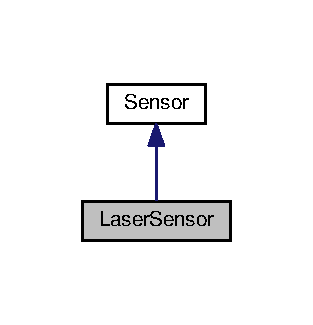
\includegraphics[width=150pt]{classLaserSensor__inherit__graph}
\end{center}
\end{figure}


Collaboration diagram for Laser\-Sensor\-:
\nopagebreak
\begin{figure}[H]
\begin{center}
\leavevmode
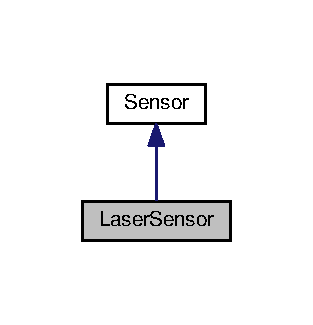
\includegraphics[width=150pt]{classLaserSensor__coll__graph}
\end{center}
\end{figure}
\subsection*{Public Member Functions}
\begin{DoxyCompactItemize}
\item 
\hyperlink{classLaserSensor_a1e40e17c9f636bc41f5612d09480aca4}{Laser\-Sensor} ()
\begin{DoxyCompactList}\small\item\em Class Constructor. \end{DoxyCompactList}\item 
virtual void \hyperlink{classLaserSensor_a1137c622e564b5706e6f36e253c2828b}{init\-Driver} (int number\-Of\-Sensors, int gain, int max\-Range)
\begin{DoxyCompactList}\small\item\em Initiates Laser \hyperlink{classSensor}{Sensor} Driver. \end{DoxyCompactList}\item 
virtual std\-::vector$<$ int $>$ \hyperlink{classLaserSensor_a1660841aa809bc22abc607780bf832b0}{get\-Sensor\-Data} ()
\begin{DoxyCompactList}\small\item\em Retrieves the Laser \hyperlink{classSensor}{Sensor} data. \end{DoxyCompactList}\item 
virtual void \hyperlink{classLaserSensor_a87ed0b803f91e74752a9097c594bcb0a}{generate\-Sensor\-Data} ()
\begin{DoxyCompactList}\small\item\em Generates the Laser \hyperlink{classSensor}{Sensor} data. \end{DoxyCompactList}\item 
virtual void \hyperlink{classLaserSensor_aa2edc4c57398799497859ab9373e9aa5}{parse\-Sensor\-Data} (std\-::vector$<$ int $>$ data)
\begin{DoxyCompactList}\small\item\em Parses the Laser \hyperlink{classSensor}{Sensor} data vector into individual variables. \end{DoxyCompactList}\item 
virtual void \hyperlink{classLaserSensor_ac6b53151004470fc1aba53be913db293}{set\-Sensor\-Type} ()
\begin{DoxyCompactList}\small\item\em Sets the \hyperlink{classSensor}{Sensor} type as Laser. \end{DoxyCompactList}\item 
virtual void \hyperlink{classLaserSensor_a04cc4baee499328b9f781edf050c092e}{set\-Maximum\-Range} (int max\-Range)
\begin{DoxyCompactList}\small\item\em Sets the maximum range of the Laser \hyperlink{classSensor}{Sensor}. \end{DoxyCompactList}\item 
virtual void \hyperlink{classLaserSensor_a79c788c37d423f350108c86666b385cb}{set\-Gain} (int gain)
\begin{DoxyCompactList}\small\item\em Sets the gain of the Laser \hyperlink{classSensor}{Sensor}. \end{DoxyCompactList}\item 
virtual std\-::string \hyperlink{classLaserSensor_aa94501358ead1126fe74e8ccaa5e83cb}{get\-Sensor\-Type} ()
\begin{DoxyCompactList}\small\item\em Retrieves the \hyperlink{classSensor}{Sensor} type\-: laser. \end{DoxyCompactList}\item 
virtual void \hyperlink{classLaserSensor_a4ce1bdb6167453f776413bcf62669562}{set\-Number\-Of\-Sensors} (int number)
\begin{DoxyCompactList}\small\item\em Configures the number of laser sensors to be used (4) \end{DoxyCompactList}\item 
virtual void \hyperlink{classLaserSensor_a186eb69518339ef4ba33e8e190a39428}{set\-Sensor\-Device\-I\-D} (int number\-Of\-Devices)
\begin{DoxyCompactList}\small\item\em Sets the device I\-Ds of the laser sensors. \end{DoxyCompactList}\item 
virtual void \hyperlink{classLaserSensor_a7b1301e42da81092ef4b16fcec3ece62}{get\-Sensor\-Device\-I\-D} ()
\begin{DoxyCompactList}\small\item\em Prints to the screen the device I\-Ds of the laser sensors. \end{DoxyCompactList}\item 
virtual void \hyperlink{classLaserSensor_a3be8d859cdab60a5e32c0855e5be928e}{get\-Time\-Stamp} ()
\begin{DoxyCompactList}\small\item\em Prints to the screen the laser sensor readings time stamp. \end{DoxyCompactList}\end{DoxyCompactItemize}


\subsection{Constructor \& Destructor Documentation}
\hypertarget{classLaserSensor_a1e40e17c9f636bc41f5612d09480aca4}{\index{Laser\-Sensor@{Laser\-Sensor}!Laser\-Sensor@{Laser\-Sensor}}
\index{Laser\-Sensor@{Laser\-Sensor}!LaserSensor@{Laser\-Sensor}}
\subsubsection[{Laser\-Sensor}]{\setlength{\rightskip}{0pt plus 5cm}Laser\-Sensor\-::\-Laser\-Sensor (
\begin{DoxyParamCaption}
{}
\end{DoxyParamCaption}
)}}\label{classLaserSensor_a1e40e17c9f636bc41f5612d09480aca4}


Class Constructor. 


\begin{DoxyCode}
10                          \{
11   numberOfSensors = 0;
12   laserSensorFront = 0;
13   laserSensorBack = 0;
14   laserSensorLeft = 0;
15   laserSensorRight = 0;
16   sensorGain = 0;
17   sensorMaximumRange = 0;
18 \}
\end{DoxyCode}


\subsection{Member Function Documentation}
\hypertarget{classLaserSensor_a87ed0b803f91e74752a9097c594bcb0a}{\index{Laser\-Sensor@{Laser\-Sensor}!generate\-Sensor\-Data@{generate\-Sensor\-Data}}
\index{generate\-Sensor\-Data@{generate\-Sensor\-Data}!LaserSensor@{Laser\-Sensor}}
\subsubsection[{generate\-Sensor\-Data}]{\setlength{\rightskip}{0pt plus 5cm}void Laser\-Sensor\-::generate\-Sensor\-Data (
\begin{DoxyParamCaption}
{}
\end{DoxyParamCaption}
)\hspace{0.3cm}{\ttfamily [virtual]}}}\label{classLaserSensor_a87ed0b803f91e74752a9097c594bcb0a}


Generates the Laser \hyperlink{classSensor}{Sensor} data. 


\begin{DoxyParams}{Parameters}
{\em none} & \\
\hline
\end{DoxyParams}
\begin{DoxyReturn}{Returns}
void function does not return anything 
\end{DoxyReturn}


Implements \hyperlink{classSensor_a1cabdc10d3319abeaa8db56724fa36e5}{Sensor}.


\begin{DoxyCode}
53                                      \{
54   std::random\_device rnd;
55   std::mt19937 gen(rnd());
56   std::uniform\_int\_distribution<> dist(1,100);
57   \textcolor{keywordflow}{for}(\textcolor{keyword}{auto} i=0; i < numberOfSensors; i++)
58     sensorData.push\_back(dist(gen));
59   \textcolor{keywordflow}{for}(\textcolor{keyword}{auto} n:sensorData)
60     std::cout << \hyperlink{classLaserSensor_aa94501358ead1126fe74e8ccaa5e83cb}{LaserSensor::getSensorType}() << \textcolor{stringliteral}{" Sensor = "} << n << std::endl;
61 \}
\end{DoxyCode}
\hypertarget{classLaserSensor_a1660841aa809bc22abc607780bf832b0}{\index{Laser\-Sensor@{Laser\-Sensor}!get\-Sensor\-Data@{get\-Sensor\-Data}}
\index{get\-Sensor\-Data@{get\-Sensor\-Data}!LaserSensor@{Laser\-Sensor}}
\subsubsection[{get\-Sensor\-Data}]{\setlength{\rightskip}{0pt plus 5cm}std\-::vector$<$ int $>$ Laser\-Sensor\-::get\-Sensor\-Data (
\begin{DoxyParamCaption}
{}
\end{DoxyParamCaption}
)\hspace{0.3cm}{\ttfamily [virtual]}}}\label{classLaserSensor_a1660841aa809bc22abc607780bf832b0}


Retrieves the Laser \hyperlink{classSensor}{Sensor} data. 


\begin{DoxyParams}{Parameters}
{\em none} & \\
\hline
\end{DoxyParams}
\begin{DoxyReturn}{Returns}
vector$<$int$>$ vector containing 4 sensor readings 
\end{DoxyReturn}


Implements \hyperlink{classSensor_a795dda4f99ae87b9d66c3c5a07722d1b}{Sensor}.


\begin{DoxyCode}
49                                           \{
50   \textcolor{keywordflow}{return} sensorData;
51 \}
\end{DoxyCode}
\hypertarget{classLaserSensor_a7b1301e42da81092ef4b16fcec3ece62}{\index{Laser\-Sensor@{Laser\-Sensor}!get\-Sensor\-Device\-I\-D@{get\-Sensor\-Device\-I\-D}}
\index{get\-Sensor\-Device\-I\-D@{get\-Sensor\-Device\-I\-D}!LaserSensor@{Laser\-Sensor}}
\subsubsection[{get\-Sensor\-Device\-I\-D}]{\setlength{\rightskip}{0pt plus 5cm}void Laser\-Sensor\-::get\-Sensor\-Device\-I\-D (
\begin{DoxyParamCaption}
{}
\end{DoxyParamCaption}
)\hspace{0.3cm}{\ttfamily [virtual]}}}\label{classLaserSensor_a7b1301e42da81092ef4b16fcec3ece62}


Prints to the screen the device I\-Ds of the laser sensors. 


\begin{DoxyParams}{Parameters}
{\em none} & \\
\hline
\end{DoxyParams}
\begin{DoxyReturn}{Returns}
void function does not return anything 
\end{DoxyReturn}


Implements \hyperlink{classSensor_af7ff987e1f0f6b7c4acf2910212fde95}{Sensor}.


\begin{DoxyCode}
95                                     \{
96   std::cout <<\textcolor{stringliteral}{"Sensor Front device ID : "} << deviceID.at(0) << std::endl;
97   std::cout <<\textcolor{stringliteral}{"Sensor Back  device ID : "} << deviceID.at(1) << std::endl;
98   std::cout <<\textcolor{stringliteral}{"Sensor Left  device ID : "} << deviceID.at(2) << std::endl;
99   std::cout <<\textcolor{stringliteral}{"Sensor Right device ID : "} << deviceID.at(3) << std::endl;
100 \}
\end{DoxyCode}
\hypertarget{classLaserSensor_aa94501358ead1126fe74e8ccaa5e83cb}{\index{Laser\-Sensor@{Laser\-Sensor}!get\-Sensor\-Type@{get\-Sensor\-Type}}
\index{get\-Sensor\-Type@{get\-Sensor\-Type}!LaserSensor@{Laser\-Sensor}}
\subsubsection[{get\-Sensor\-Type}]{\setlength{\rightskip}{0pt plus 5cm}std\-::string Laser\-Sensor\-::get\-Sensor\-Type (
\begin{DoxyParamCaption}
{}
\end{DoxyParamCaption}
)\hspace{0.3cm}{\ttfamily [virtual]}}}\label{classLaserSensor_aa94501358ead1126fe74e8ccaa5e83cb}


Retrieves the \hyperlink{classSensor}{Sensor} type\-: laser. 


\begin{DoxyParams}{Parameters}
{\em none} & \\
\hline
\end{DoxyParams}
\begin{DoxyReturn}{Returns}
string Contains the sensor type (laser) 
\end{DoxyReturn}


Implements \hyperlink{classSensor_a6cf36c37e69761711982fed5d14aeb4e}{Sensor}.


\begin{DoxyCode}
78                                      \{
79   \textcolor{keywordflow}{return} sensorType;
80 \}
\end{DoxyCode}
\hypertarget{classLaserSensor_a3be8d859cdab60a5e32c0855e5be928e}{\index{Laser\-Sensor@{Laser\-Sensor}!get\-Time\-Stamp@{get\-Time\-Stamp}}
\index{get\-Time\-Stamp@{get\-Time\-Stamp}!LaserSensor@{Laser\-Sensor}}
\subsubsection[{get\-Time\-Stamp}]{\setlength{\rightskip}{0pt plus 5cm}void Laser\-Sensor\-::get\-Time\-Stamp (
\begin{DoxyParamCaption}
{}
\end{DoxyParamCaption}
)\hspace{0.3cm}{\ttfamily [virtual]}}}\label{classLaserSensor_a3be8d859cdab60a5e32c0855e5be928e}


Prints to the screen the laser sensor readings time stamp. 


\begin{DoxyParams}{Parameters}
{\em none} & \\
\hline
\end{DoxyParams}
\begin{DoxyReturn}{Returns}
void function does not return anything 
\end{DoxyReturn}


Implements \hyperlink{classSensor_a8c6ceb519eb8720a0e9cedd84624a7ff}{Sensor}.


\begin{DoxyCode}
102                                \{
103   \textcolor{keyword}{auto} now = std::chrono::system\_clock::now();
104   \textcolor{keyword}{auto} nowC = std::chrono::system\_clock::to\_time\_t(now);
105   std::cout << \textcolor{stringliteral}{"Time stamp = "} << std::ctime(&nowC) << std::endl;
106 \}
\end{DoxyCode}
\hypertarget{classLaserSensor_a1137c622e564b5706e6f36e253c2828b}{\index{Laser\-Sensor@{Laser\-Sensor}!init\-Driver@{init\-Driver}}
\index{init\-Driver@{init\-Driver}!LaserSensor@{Laser\-Sensor}}
\subsubsection[{init\-Driver}]{\setlength{\rightskip}{0pt plus 5cm}void Laser\-Sensor\-::init\-Driver (
\begin{DoxyParamCaption}
\item[{int}]{number\-Of\-Sensors, }
\item[{int}]{gain, }
\item[{int}]{max\-Range}
\end{DoxyParamCaption}
)\hspace{0.3cm}{\ttfamily [virtual]}}}\label{classLaserSensor_a1137c622e564b5706e6f36e253c2828b}


Initiates Laser \hyperlink{classSensor}{Sensor} Driver. 


\begin{DoxyParams}{Parameters}
{\em number\-Of\-Sensors} & sets the number of sensors in the module \\
\hline
{\em gain} & sets the gain of the module \\
\hline
{\em max\-Range} & sets the maximum range of the module \\
\hline
\end{DoxyParams}
\begin{DoxyReturn}{Returns}
void function does not return anything
\end{DoxyReturn}
This method executes all initialization functions for the module. 

Implements \hyperlink{classSensor_a12851eb9413ee61c2d694b4168e365fd}{Sensor}.


\begin{DoxyCode}
20                                                                        \{
21   \textcolor{keywordflow}{if} (std::isless(numberOfSensors,0) || std::isless(gain,0) || std::isless(maxRange,0))
22     \textcolor{keywordflow}{throw} std::domain\_error(\textcolor{stringliteral}{"Negative arguments are invalid"});
23   std::cout <<\textcolor{stringliteral}{"=====================================\(\backslash\)n"};
24   std::cout <<\textcolor{stringliteral}{"Initializing Laser Sensors..........!\(\backslash\)n"};
25   std::cout <<\textcolor{stringliteral}{".....................................\(\backslash\)n"};
26   \hyperlink{classLaserSensor_ac6b53151004470fc1aba53be913db293}{LaserSensor::setSensorType}();
27   \hyperlink{classLaserSensor_a79c788c37d423f350108c86666b385cb}{LaserSensor::setGain}(gain);
28   \hyperlink{classLaserSensor_a04cc4baee499328b9f781edf050c092e}{LaserSensor::setMaximumRange}(maxRange);
29   \hyperlink{classLaserSensor_a186eb69518339ef4ba33e8e190a39428}{LaserSensor::setSensorDeviceID}(numberOfSensors);
30   \hyperlink{classLaserSensor_a4ce1bdb6167453f776413bcf62669562}{LaserSensor::setNumberOfSensors}(numberOfSensors);
31   \hyperlink{classLaserSensor_a7b1301e42da81092ef4b16fcec3ece62}{LaserSensor::getSensorDeviceID}();
32   std::cout <<\textcolor{stringliteral}{".....................................\(\backslash\)n"};
33 \}
\end{DoxyCode}
\hypertarget{classLaserSensor_aa2edc4c57398799497859ab9373e9aa5}{\index{Laser\-Sensor@{Laser\-Sensor}!parse\-Sensor\-Data@{parse\-Sensor\-Data}}
\index{parse\-Sensor\-Data@{parse\-Sensor\-Data}!LaserSensor@{Laser\-Sensor}}
\subsubsection[{parse\-Sensor\-Data}]{\setlength{\rightskip}{0pt plus 5cm}void Laser\-Sensor\-::parse\-Sensor\-Data (
\begin{DoxyParamCaption}
\item[{std\-::vector$<$ int $>$}]{data}
\end{DoxyParamCaption}
)\hspace{0.3cm}{\ttfamily [virtual]}}}\label{classLaserSensor_aa2edc4c57398799497859ab9373e9aa5}


Parses the Laser \hyperlink{classSensor}{Sensor} data vector into individual variables. 


\begin{DoxyParams}{Parameters}
{\em data} & vector containing 4 integer readings \\
\hline
\end{DoxyParams}
\begin{DoxyReturn}{Returns}
void function does not return anything 
\end{DoxyReturn}


Implements \hyperlink{classSensor_a32f0d1754f66bdb26bbece93e05b9a44}{Sensor}.


\begin{DoxyCode}
62                                                      \{
63   laserSensorFront = data.at(0);
64   std::cout <<\textcolor{stringliteral}{"Sensor Front value = "} << laserSensorFront << std::endl;
65   laserSensorBack  = data.at(1);
66   std::cout <<\textcolor{stringliteral}{"Sensor Back value = "} << laserSensorBack << std::endl;   
67   laserSensorLeft  = data.at(2);
68   std::cout <<\textcolor{stringliteral}{"Sensor Left value = "} << laserSensorLeft << std::endl;
69   laserSensorRight = data.at(3);
70   std::cout <<\textcolor{stringliteral}{"Sensor Right value = "} << laserSensorRight << std::endl;
71 \}
\end{DoxyCode}
\hypertarget{classLaserSensor_a79c788c37d423f350108c86666b385cb}{\index{Laser\-Sensor@{Laser\-Sensor}!set\-Gain@{set\-Gain}}
\index{set\-Gain@{set\-Gain}!LaserSensor@{Laser\-Sensor}}
\subsubsection[{set\-Gain}]{\setlength{\rightskip}{0pt plus 5cm}void Laser\-Sensor\-::set\-Gain (
\begin{DoxyParamCaption}
\item[{int}]{gain}
\end{DoxyParamCaption}
)\hspace{0.3cm}{\ttfamily [virtual]}}}\label{classLaserSensor_a79c788c37d423f350108c86666b385cb}


Sets the gain of the Laser \hyperlink{classSensor}{Sensor}. 


\begin{DoxyParams}{Parameters}
{\em gain} & sensor gain \\
\hline
\end{DoxyParams}
\begin{DoxyReturn}{Returns}
void function does not return anything 
\end{DoxyReturn}

\begin{DoxyCode}
42                                   \{
43   \textcolor{keywordflow}{if} (std::isless(gain,0))
44     \textcolor{keywordflow}{throw} std::domain\_error(\textcolor{stringliteral}{"Negative gain not allowed"});
45   sensorGain = gain;
46   std::cout <<\textcolor{stringliteral}{"Sensor gain : "}<<sensorGain<<std::endl;
47 \}
\end{DoxyCode}
\hypertarget{classLaserSensor_a04cc4baee499328b9f781edf050c092e}{\index{Laser\-Sensor@{Laser\-Sensor}!set\-Maximum\-Range@{set\-Maximum\-Range}}
\index{set\-Maximum\-Range@{set\-Maximum\-Range}!LaserSensor@{Laser\-Sensor}}
\subsubsection[{set\-Maximum\-Range}]{\setlength{\rightskip}{0pt plus 5cm}void Laser\-Sensor\-::set\-Maximum\-Range (
\begin{DoxyParamCaption}
\item[{int}]{max\-Range}
\end{DoxyParamCaption}
)\hspace{0.3cm}{\ttfamily [virtual]}}}\label{classLaserSensor_a04cc4baee499328b9f781edf050c092e}


Sets the maximum range of the Laser \hyperlink{classSensor}{Sensor}. 


\begin{DoxyParams}{Parameters}
{\em max\-Range} & maximum range \\
\hline
\end{DoxyParams}
\begin{DoxyReturn}{Returns}
void function does not return anything 
\end{DoxyReturn}

\begin{DoxyCode}
35                                               \{
36   \textcolor{keywordflow}{if} (std::isless(maxRange,0))
37     \textcolor{keywordflow}{throw} std::domain\_error(\textcolor{stringliteral}{"Negative range not allowed"});
38   sensorMaximumRange = maxRange;
39   std::cout <<\textcolor{stringliteral}{"Sensor Maximum range : "}<<sensorMaximumRange<<std::endl;
40 \}
\end{DoxyCode}
\hypertarget{classLaserSensor_a4ce1bdb6167453f776413bcf62669562}{\index{Laser\-Sensor@{Laser\-Sensor}!set\-Number\-Of\-Sensors@{set\-Number\-Of\-Sensors}}
\index{set\-Number\-Of\-Sensors@{set\-Number\-Of\-Sensors}!LaserSensor@{Laser\-Sensor}}
\subsubsection[{set\-Number\-Of\-Sensors}]{\setlength{\rightskip}{0pt plus 5cm}void Laser\-Sensor\-::set\-Number\-Of\-Sensors (
\begin{DoxyParamCaption}
\item[{int}]{number}
\end{DoxyParamCaption}
)\hspace{0.3cm}{\ttfamily [virtual]}}}\label{classLaserSensor_a4ce1bdb6167453f776413bcf62669562}


Configures the number of laser sensors to be used (4) 


\begin{DoxyParams}{Parameters}
{\em number} & number of sensors \\
\hline
\end{DoxyParams}
\begin{DoxyReturn}{Returns}
void function does not return anything 
\end{DoxyReturn}


Implements \hyperlink{classSensor_a5372c229e1bf77d70d48506af8abd351}{Sensor}.


\begin{DoxyCode}
82                                                \{
83   \textcolor{keywordflow}{if} (std::isless(number,0))
84     \textcolor{keywordflow}{throw} std::domain\_error(\textcolor{stringliteral}{"Negative arguments are invalid"});
85   numberOfSensors = number;
86 \}
\end{DoxyCode}
\hypertarget{classLaserSensor_a186eb69518339ef4ba33e8e190a39428}{\index{Laser\-Sensor@{Laser\-Sensor}!set\-Sensor\-Device\-I\-D@{set\-Sensor\-Device\-I\-D}}
\index{set\-Sensor\-Device\-I\-D@{set\-Sensor\-Device\-I\-D}!LaserSensor@{Laser\-Sensor}}
\subsubsection[{set\-Sensor\-Device\-I\-D}]{\setlength{\rightskip}{0pt plus 5cm}void Laser\-Sensor\-::set\-Sensor\-Device\-I\-D (
\begin{DoxyParamCaption}
\item[{int}]{number\-Of\-Devices}
\end{DoxyParamCaption}
)\hspace{0.3cm}{\ttfamily [virtual]}}}\label{classLaserSensor_a186eb69518339ef4ba33e8e190a39428}


Sets the device I\-Ds of the laser sensors. 


\begin{DoxyParams}{Parameters}
{\em number\-Of\-Devices} & number of devices \\
\hline
\end{DoxyParams}
\begin{DoxyReturn}{Returns}
void function does not return anything 
\end{DoxyReturn}


Implements \hyperlink{classSensor_a3a7ad3cdc0e9a5ef6f5ce684c7a0c59a}{Sensor}.


\begin{DoxyCode}
88                                                        \{
89   \textcolor{keywordflow}{if} (std::isless(numberOfDevices,0))
90     \textcolor{keywordflow}{throw} std::domain\_error(\textcolor{stringliteral}{"Negative arguments are invalid"});
91   \textcolor{keywordflow}{for} (\textcolor{keyword}{auto} i =1; i <= numberOfDevices; i++)
92     deviceID.push\_back((i*10)+40);
93 \}
\end{DoxyCode}
\hypertarget{classLaserSensor_ac6b53151004470fc1aba53be913db293}{\index{Laser\-Sensor@{Laser\-Sensor}!set\-Sensor\-Type@{set\-Sensor\-Type}}
\index{set\-Sensor\-Type@{set\-Sensor\-Type}!LaserSensor@{Laser\-Sensor}}
\subsubsection[{set\-Sensor\-Type}]{\setlength{\rightskip}{0pt plus 5cm}void Laser\-Sensor\-::set\-Sensor\-Type (
\begin{DoxyParamCaption}
{}
\end{DoxyParamCaption}
)\hspace{0.3cm}{\ttfamily [virtual]}}}\label{classLaserSensor_ac6b53151004470fc1aba53be913db293}


Sets the \hyperlink{classSensor}{Sensor} type as Laser. 


\begin{DoxyParams}{Parameters}
{\em none} & \\
\hline
\end{DoxyParams}
\begin{DoxyReturn}{Returns}
void function does not return anything 
\end{DoxyReturn}


Implements \hyperlink{classSensor_a53daf1760d09355a8d3846addc53bd6e}{Sensor}.


\begin{DoxyCode}
73                                 \{
74   sensorType = \textcolor{stringliteral}{"Laser"};
75   std::cout <<\textcolor{stringliteral}{"Sensor Type : "} << \hyperlink{classLaserSensor_aa94501358ead1126fe74e8ccaa5e83cb}{LaserSensor::getSensorType}() << std::endl;
76 \}
\end{DoxyCode}


The documentation for this class was generated from the following files\-:\begin{DoxyCompactItemize}
\item 
Obstacle\-Avoidance/include/\hyperlink{LaserSensor_8h}{Laser\-Sensor.\-h}\item 
Obstacle\-Avoidance/app/\hyperlink{LaserSensor_8cpp}{Laser\-Sensor.\-cpp}\end{DoxyCompactItemize}

\hypertarget{classMotorController}{\section{Motor\-Controller Class Reference}
\label{classMotorController}\index{Motor\-Controller@{Motor\-Controller}}
}


{\ttfamily \#include $<$Motor\-Controller.\-h$>$}

\subsection*{Public Member Functions}
\begin{DoxyCompactItemize}
\item 
\hyperlink{classMotorController_a1c32db157ba4b6dba1f2d6bc8891f16d}{Motor\-Controller} ()
\begin{DoxyCompactList}\small\item\em Class constructor. \end{DoxyCompactList}\item 
void \hyperlink{classMotorController_a56ae5e4c44399b8afe94eb721514dd5e}{initialize\-Motor\-Controller} ()
\begin{DoxyCompactList}\small\item\em Initializes motor controller. \end{DoxyCompactList}\item 
void \hyperlink{classMotorController_ab0dffd70556dbab55aa990673e6dc5f8}{move\-Forward} (int)
\begin{DoxyCompactList}\small\item\em Moves forward. \end{DoxyCompactList}\item 
void \hyperlink{classMotorController_a3ad21d7cff7b0c3c6700b2755b1df2d2}{move\-Backwards} (int)
\begin{DoxyCompactList}\small\item\em Moves backwards. \end{DoxyCompactList}\item 
void \hyperlink{classMotorController_a4c3beafe5316cd08fd44845e20ec7151}{move\-Left} (int)
\begin{DoxyCompactList}\small\item\em Moves left. \end{DoxyCompactList}\item 
void \hyperlink{classMotorController_aa1586060f2ee0f66e83d30c897a1cdb4}{move\-Right} (int)
\begin{DoxyCompactList}\small\item\em Moves right. \end{DoxyCompactList}\end{DoxyCompactItemize}


\subsection{Constructor \& Destructor Documentation}
\hypertarget{classMotorController_a1c32db157ba4b6dba1f2d6bc8891f16d}{\index{Motor\-Controller@{Motor\-Controller}!Motor\-Controller@{Motor\-Controller}}
\index{Motor\-Controller@{Motor\-Controller}!MotorController@{Motor\-Controller}}
\subsubsection[{Motor\-Controller}]{\setlength{\rightskip}{0pt plus 5cm}Motor\-Controller\-::\-Motor\-Controller (
\begin{DoxyParamCaption}
{}
\end{DoxyParamCaption}
)}}\label{classMotorController_a1c32db157ba4b6dba1f2d6bc8891f16d}


Class constructor. 


\begin{DoxyCode}
10                                  \{
11   fwdSpeed  = 0;
12   backSpeed = 0;
13   leftSpeed = 0;
14   rightSpeed = 0;
15 \}
\end{DoxyCode}


\subsection{Member Function Documentation}
\hypertarget{classMotorController_a56ae5e4c44399b8afe94eb721514dd5e}{\index{Motor\-Controller@{Motor\-Controller}!initialize\-Motor\-Controller@{initialize\-Motor\-Controller}}
\index{initialize\-Motor\-Controller@{initialize\-Motor\-Controller}!MotorController@{Motor\-Controller}}
\subsubsection[{initialize\-Motor\-Controller}]{\setlength{\rightskip}{0pt plus 5cm}void Motor\-Controller\-::initialize\-Motor\-Controller (
\begin{DoxyParamCaption}
{}
\end{DoxyParamCaption}
)}}\label{classMotorController_a56ae5e4c44399b8afe94eb721514dd5e}


Initializes motor controller. 


\begin{DoxyCode}
17                                                 \{
18   std::cout <<\textcolor{stringliteral}{"=====================================\(\backslash\)n"};
19   std::cout <<\textcolor{stringliteral}{"Initializing Motor Controller.......!\(\backslash\)n"};
20   std::cout <<\textcolor{stringliteral}{".....................................\(\backslash\)n"};
21   fwdSpeed = 0;
22   std::cout <<\textcolor{stringliteral}{"Forward Speed = "} << fwdSpeed << \textcolor{stringliteral}{" mi/h\(\backslash\)n"};
23   backSpeed = 0;
24   std::cout <<\textcolor{stringliteral}{"Backward Speed = "} << backSpeed << \textcolor{stringliteral}{" mi/h\(\backslash\)n"};
25   leftSpeed = 0;
26   std::cout <<\textcolor{stringliteral}{"Left Speed = "}<< leftSpeed <<\textcolor{stringliteral}{" mi/h\(\backslash\)n"};
27   rightSpeed = 0;
28   std::cout <<\textcolor{stringliteral}{"Right Speed = "}<< rightSpeed <<\textcolor{stringliteral}{" mi/h\(\backslash\)n"};
29 \}
\end{DoxyCode}
\hypertarget{classMotorController_a3ad21d7cff7b0c3c6700b2755b1df2d2}{\index{Motor\-Controller@{Motor\-Controller}!move\-Backwards@{move\-Backwards}}
\index{move\-Backwards@{move\-Backwards}!MotorController@{Motor\-Controller}}
\subsubsection[{move\-Backwards}]{\setlength{\rightskip}{0pt plus 5cm}void Motor\-Controller\-::move\-Backwards (
\begin{DoxyParamCaption}
\item[{int}]{speed}
\end{DoxyParamCaption}
)}}\label{classMotorController_a3ad21d7cff7b0c3c6700b2755b1df2d2}


Moves backwards. 


\begin{DoxyCode}
36                                              \{
37   backSpeed = speed;
38   std::cout <<\textcolor{stringliteral}{"Moving backwards at "}<< backSpeed <<\textcolor{stringliteral}{" mi/h\(\backslash\)n"};
39 \}
\end{DoxyCode}
\hypertarget{classMotorController_ab0dffd70556dbab55aa990673e6dc5f8}{\index{Motor\-Controller@{Motor\-Controller}!move\-Forward@{move\-Forward}}
\index{move\-Forward@{move\-Forward}!MotorController@{Motor\-Controller}}
\subsubsection[{move\-Forward}]{\setlength{\rightskip}{0pt plus 5cm}void Motor\-Controller\-::move\-Forward (
\begin{DoxyParamCaption}
\item[{int}]{speed}
\end{DoxyParamCaption}
)}}\label{classMotorController_ab0dffd70556dbab55aa990673e6dc5f8}


Moves forward. 


\begin{DoxyCode}
31                                            \{
32   fwdSpeed = speed;
33   std::cout <<\textcolor{stringliteral}{"Moving forward at "}<< fwdSpeed <<\textcolor{stringliteral}{" mi/h\(\backslash\)n"};
34 \}
\end{DoxyCode}
\hypertarget{classMotorController_a4c3beafe5316cd08fd44845e20ec7151}{\index{Motor\-Controller@{Motor\-Controller}!move\-Left@{move\-Left}}
\index{move\-Left@{move\-Left}!MotorController@{Motor\-Controller}}
\subsubsection[{move\-Left}]{\setlength{\rightskip}{0pt plus 5cm}void Motor\-Controller\-::move\-Left (
\begin{DoxyParamCaption}
\item[{int}]{speed}
\end{DoxyParamCaption}
)}}\label{classMotorController_a4c3beafe5316cd08fd44845e20ec7151}


Moves left. 


\begin{DoxyCode}
41                                         \{
42   leftSpeed = speed;
43   std::cout <<\textcolor{stringliteral}{"Moving left at "}<< leftSpeed <<\textcolor{stringliteral}{" mi/h\(\backslash\)n"};
44 \}
\end{DoxyCode}
\hypertarget{classMotorController_aa1586060f2ee0f66e83d30c897a1cdb4}{\index{Motor\-Controller@{Motor\-Controller}!move\-Right@{move\-Right}}
\index{move\-Right@{move\-Right}!MotorController@{Motor\-Controller}}
\subsubsection[{move\-Right}]{\setlength{\rightskip}{0pt plus 5cm}void Motor\-Controller\-::move\-Right (
\begin{DoxyParamCaption}
\item[{int}]{speed}
\end{DoxyParamCaption}
)}}\label{classMotorController_aa1586060f2ee0f66e83d30c897a1cdb4}


Moves right. 


\begin{DoxyCode}
46                                          \{
47   rightSpeed = speed;
48   std::cout <<\textcolor{stringliteral}{"Moving right at "}<< rightSpeed <<\textcolor{stringliteral}{" mi/h\(\backslash\)n"};
49 \}
\end{DoxyCode}


The documentation for this class was generated from the following files\-:\begin{DoxyCompactItemize}
\item 
Obstacle\-Avoidance/include/\hyperlink{MotorController_8h}{Motor\-Controller.\-h}\item 
Obstacle\-Avoidance/app/\hyperlink{MotorController_8cpp}{Motor\-Controller.\-cpp}\end{DoxyCompactItemize}

\hypertarget{classObstacleAvoidance}{\section{Obstacle\-Avoidance Class Reference}
\label{classObstacleAvoidance}\index{Obstacle\-Avoidance@{Obstacle\-Avoidance}}
}


{\ttfamily \#include $<$Obstacle\-Avoidance\-Module.\-h$>$}

\subsection*{Public Member Functions}
\begin{DoxyCompactItemize}
\item 
\hyperlink{classObstacleAvoidance_adff25e3149ac860f48af277913c6e51e}{Obstacle\-Avoidance} ()
\begin{DoxyCompactList}\small\item\em class constructor \end{DoxyCompactList}\item 
void \hyperlink{classObstacleAvoidance_a05040b1d9096fa315e439a0a9cd3a0e3}{detect\-Obstacle} (int front, int back, int left, int right)
\begin{DoxyCompactList}\small\item\em Detects obstacles. \end{DoxyCompactList}\item 
void \hyperlink{classObstacleAvoidance_a646828a87a384074b80df0a0ff1320ec}{trn\-On\-Off\-Avoid} (int \&front\-Spd, int \&back\-Spd, int \&left\-Spd, int \&right\-Spd)
\begin{DoxyCompactList}\small\item\em Overrides speed. \end{DoxyCompactList}\end{DoxyCompactItemize}


\subsection{Constructor \& Destructor Documentation}
\hypertarget{classObstacleAvoidance_adff25e3149ac860f48af277913c6e51e}{\index{Obstacle\-Avoidance@{Obstacle\-Avoidance}!Obstacle\-Avoidance@{Obstacle\-Avoidance}}
\index{Obstacle\-Avoidance@{Obstacle\-Avoidance}!ObstacleAvoidance@{Obstacle\-Avoidance}}
\subsubsection[{Obstacle\-Avoidance}]{\setlength{\rightskip}{0pt plus 5cm}Obstacle\-Avoidance\-::\-Obstacle\-Avoidance (
\begin{DoxyParamCaption}
{}
\end{DoxyParamCaption}
)}}\label{classObstacleAvoidance_adff25e3149ac860f48af277913c6e51e}


class constructor 


\begin{DoxyCode}
10                                      \{
11   frontObstacle = \textcolor{keyword}{false};
12   backObstacle = \textcolor{keyword}{false};
13   leftObstacle = \textcolor{keyword}{false};
14   rightObstacle = \textcolor{keyword}{false};
15 \}
\end{DoxyCode}


\subsection{Member Function Documentation}
\hypertarget{classObstacleAvoidance_a05040b1d9096fa315e439a0a9cd3a0e3}{\index{Obstacle\-Avoidance@{Obstacle\-Avoidance}!detect\-Obstacle@{detect\-Obstacle}}
\index{detect\-Obstacle@{detect\-Obstacle}!ObstacleAvoidance@{Obstacle\-Avoidance}}
\subsubsection[{detect\-Obstacle}]{\setlength{\rightskip}{0pt plus 5cm}void Obstacle\-Avoidance\-::detect\-Obstacle (
\begin{DoxyParamCaption}
\item[{int}]{front, }
\item[{int}]{back, }
\item[{int}]{left, }
\item[{int}]{right}
\end{DoxyParamCaption}
)}}\label{classObstacleAvoidance_a05040b1d9096fa315e439a0a9cd3a0e3}


Detects obstacles. 


\begin{DoxyParams}{Parameters}
{\em front} & front sensor reading \\
\hline
{\em back} & back sensor reading \\
\hline
{\em left} & left sensor reading \\
\hline
{\em right} & right sensor reading \\
\hline
\end{DoxyParams}
\begin{DoxyReturn}{Returns}
void function does not return anything 
\end{DoxyReturn}

\begin{DoxyCode}
17                                                                             \{
18   \textcolor{keywordflow}{if} (std::isless(front,0) || std::isless(back,0) || std::isless(left,0) || std::isless(right,0))
19     \textcolor{keywordflow}{throw} std::domain\_error(\textcolor{stringliteral}{"Negative arguments are invalid"});
20   \textcolor{keywordflow}{if}(front <= 25) \{
21     std::cout << \textcolor{stringliteral}{"Object Detected in forward path\(\backslash\)n"};
22     frontObstacle = \textcolor{keyword}{true};
23   \}
24   \textcolor{keywordflow}{if}(back <= 25) \{
25     std::cout << \textcolor{stringliteral}{"Object Detected in backward path\(\backslash\)n"};
26     backObstacle = \textcolor{keyword}{true};
27   \}
28   \textcolor{keywordflow}{if}(left <= 25) \{
29     std::cout << \textcolor{stringliteral}{"Object Detected in left path\(\backslash\)n"};
30     leftObstacle = \textcolor{keyword}{true};
31   \}
32   \textcolor{keywordflow}{if}(right <= 25) \{
33     std::cout << \textcolor{stringliteral}{"Object Detected in right path\(\backslash\)n"};
34     rightObstacle = \textcolor{keyword}{true};
35   \}
36 \}
\end{DoxyCode}
\hypertarget{classObstacleAvoidance_a646828a87a384074b80df0a0ff1320ec}{\index{Obstacle\-Avoidance@{Obstacle\-Avoidance}!trn\-On\-Off\-Avoid@{trn\-On\-Off\-Avoid}}
\index{trn\-On\-Off\-Avoid@{trn\-On\-Off\-Avoid}!ObstacleAvoidance@{Obstacle\-Avoidance}}
\subsubsection[{trn\-On\-Off\-Avoid}]{\setlength{\rightskip}{0pt plus 5cm}void Obstacle\-Avoidance\-::trn\-On\-Off\-Avoid (
\begin{DoxyParamCaption}
\item[{int \&}]{front\-Spd, }
\item[{int \&}]{back\-Spd, }
\item[{int \&}]{left\-Spd, }
\item[{int \&}]{right\-Spd}
\end{DoxyParamCaption}
)}}\label{classObstacleAvoidance_a646828a87a384074b80df0a0ff1320ec}


Overrides speed. 


\begin{DoxyParams}{Parameters}
{\em front} & front speed \\
\hline
{\em back} & back speed \\
\hline
{\em left} & left speed \\
\hline
{\em right} & right speed \\
\hline
\end{DoxyParams}
\begin{DoxyReturn}{Returns}
void function does not return anything 
\end{DoxyReturn}

\begin{DoxyCode}
39                                                                                              \{
40   \textcolor{keywordflow}{if} (std::isless(frontSpd,0) || std::isless(backSpd,0) || std::isless(leftSpd,0) || std::isless(rightSpd,0
      ))
41     \textcolor{keywordflow}{throw} std::domain\_error(\textcolor{stringliteral}{"Negative arguments are invalid"});
42   \textcolor{keywordflow}{if}(frontObstacle) \{
43     frontSpd = 0;
44     std::cout << \textcolor{stringliteral}{"Overriding Forward speed to 0........!\(\backslash\)n"};
45     frontObstacle = \textcolor{keyword}{false};      
46   \}
47   \textcolor{keywordflow}{if}(backObstacle) \{
48     backSpd = 0;
49     std::cout << \textcolor{stringliteral}{"Overriding Backward speed to 0.......!\(\backslash\)n"};
50     backObstacle = \textcolor{keyword}{false};       
51     \}
52   \textcolor{keywordflow}{if}(leftObstacle) \{
53     leftSpd = 0;
54     std::cout << \textcolor{stringliteral}{"Overriding Left speed to 0...........!\(\backslash\)n"};
55     leftObstacle = \textcolor{keyword}{false};
56   \}
57   \textcolor{keywordflow}{if}(rightObstacle) \{
58     rightSpd = 0;
59     std::cout << \textcolor{stringliteral}{"Overriding Right speed to 0..........!\(\backslash\)n"};
60     leftObstacle = \textcolor{keyword}{false};   
61   \}
62 \}
\end{DoxyCode}


The documentation for this class was generated from the following files\-:\begin{DoxyCompactItemize}
\item 
Obstacle\-Avoidance/include/\hyperlink{ObstacleAvoidanceModule_8h}{Obstacle\-Avoidance\-Module.\-h}\item 
Obstacle\-Avoidance/app/\hyperlink{ObstacleAvoidanceModule_8cpp}{Obstacle\-Avoidance\-Module.\-cpp}\end{DoxyCompactItemize}

\hypertarget{classSensor}{\section{Sensor Class Reference}
\label{classSensor}\index{Sensor@{Sensor}}
}


{\ttfamily \#include $<$Sensor.\-h$>$}



Inheritance diagram for Sensor\-:
\nopagebreak
\begin{figure}[H]
\begin{center}
\leavevmode
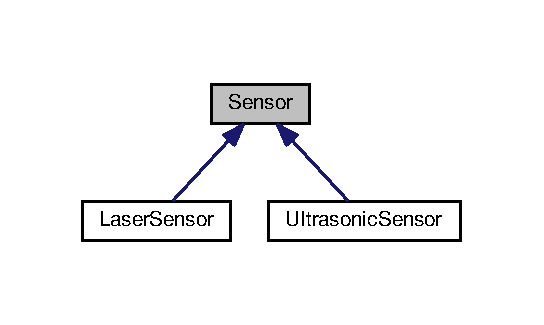
\includegraphics[width=261pt]{classSensor__inherit__graph}
\end{center}
\end{figure}
\subsection*{Public Member Functions}
\begin{DoxyCompactItemize}
\item 
virtual void \hyperlink{classSensor_a12851eb9413ee61c2d694b4168e365fd}{init\-Driver} (int number\-Of\-Sensors, int gain, int max\-Range)=0
\item 
virtual std\-::vector$<$ int $>$ \hyperlink{classSensor_a795dda4f99ae87b9d66c3c5a07722d1b}{get\-Sensor\-Data} ()=0
\item 
virtual void \hyperlink{classSensor_a1cabdc10d3319abeaa8db56724fa36e5}{generate\-Sensor\-Data} ()=0
\item 
virtual void \hyperlink{classSensor_a32f0d1754f66bdb26bbece93e05b9a44}{parse\-Sensor\-Data} (std\-::vector$<$ int $>$ data)=0
\item 
virtual void \hyperlink{classSensor_a53daf1760d09355a8d3846addc53bd6e}{set\-Sensor\-Type} ()=0
\item 
virtual std\-::string \hyperlink{classSensor_a6cf36c37e69761711982fed5d14aeb4e}{get\-Sensor\-Type} ()=0
\item 
virtual void \hyperlink{classSensor_a5372c229e1bf77d70d48506af8abd351}{set\-Number\-Of\-Sensors} (int number)=0
\item 
virtual void \hyperlink{classSensor_af7ff987e1f0f6b7c4acf2910212fde95}{get\-Sensor\-Device\-I\-D} ()=0
\item 
virtual void \hyperlink{classSensor_a3a7ad3cdc0e9a5ef6f5ce684c7a0c59a}{set\-Sensor\-Device\-I\-D} (int number\-Of\-Devices)=0
\item 
virtual void \hyperlink{classSensor_a8c6ceb519eb8720a0e9cedd84624a7ff}{get\-Time\-Stamp} ()=0
\end{DoxyCompactItemize}


\subsection{Member Function Documentation}
\hypertarget{classSensor_a1cabdc10d3319abeaa8db56724fa36e5}{\index{Sensor@{Sensor}!generate\-Sensor\-Data@{generate\-Sensor\-Data}}
\index{generate\-Sensor\-Data@{generate\-Sensor\-Data}!Sensor@{Sensor}}
\subsubsection[{generate\-Sensor\-Data}]{\setlength{\rightskip}{0pt plus 5cm}virtual void Sensor\-::generate\-Sensor\-Data (
\begin{DoxyParamCaption}
{}
\end{DoxyParamCaption}
)\hspace{0.3cm}{\ttfamily [pure virtual]}}}\label{classSensor_a1cabdc10d3319abeaa8db56724fa36e5}


Implemented in \hyperlink{classUltrasonicSensor_a5587d9432d42a82d9f6f853b0aecddd3}{Ultrasonic\-Sensor}, and \hyperlink{classLaserSensor_a87ed0b803f91e74752a9097c594bcb0a}{Laser\-Sensor}.

\hypertarget{classSensor_a795dda4f99ae87b9d66c3c5a07722d1b}{\index{Sensor@{Sensor}!get\-Sensor\-Data@{get\-Sensor\-Data}}
\index{get\-Sensor\-Data@{get\-Sensor\-Data}!Sensor@{Sensor}}
\subsubsection[{get\-Sensor\-Data}]{\setlength{\rightskip}{0pt plus 5cm}virtual std\-::vector$<$int$>$ Sensor\-::get\-Sensor\-Data (
\begin{DoxyParamCaption}
{}
\end{DoxyParamCaption}
)\hspace{0.3cm}{\ttfamily [pure virtual]}}}\label{classSensor_a795dda4f99ae87b9d66c3c5a07722d1b}


Implemented in \hyperlink{classUltrasonicSensor_a4dab101931d788a031fe44db24d0c305}{Ultrasonic\-Sensor}, and \hyperlink{classLaserSensor_a1660841aa809bc22abc607780bf832b0}{Laser\-Sensor}.

\hypertarget{classSensor_af7ff987e1f0f6b7c4acf2910212fde95}{\index{Sensor@{Sensor}!get\-Sensor\-Device\-I\-D@{get\-Sensor\-Device\-I\-D}}
\index{get\-Sensor\-Device\-I\-D@{get\-Sensor\-Device\-I\-D}!Sensor@{Sensor}}
\subsubsection[{get\-Sensor\-Device\-I\-D}]{\setlength{\rightskip}{0pt plus 5cm}virtual void Sensor\-::get\-Sensor\-Device\-I\-D (
\begin{DoxyParamCaption}
{}
\end{DoxyParamCaption}
)\hspace{0.3cm}{\ttfamily [pure virtual]}}}\label{classSensor_af7ff987e1f0f6b7c4acf2910212fde95}


Implemented in \hyperlink{classLaserSensor_a7b1301e42da81092ef4b16fcec3ece62}{Laser\-Sensor}, and \hyperlink{classUltrasonicSensor_a1676043861eb34cb61e27002212b90cc}{Ultrasonic\-Sensor}.

\hypertarget{classSensor_a6cf36c37e69761711982fed5d14aeb4e}{\index{Sensor@{Sensor}!get\-Sensor\-Type@{get\-Sensor\-Type}}
\index{get\-Sensor\-Type@{get\-Sensor\-Type}!Sensor@{Sensor}}
\subsubsection[{get\-Sensor\-Type}]{\setlength{\rightskip}{0pt plus 5cm}virtual std\-::string Sensor\-::get\-Sensor\-Type (
\begin{DoxyParamCaption}
{}
\end{DoxyParamCaption}
)\hspace{0.3cm}{\ttfamily [pure virtual]}}}\label{classSensor_a6cf36c37e69761711982fed5d14aeb4e}


Implemented in \hyperlink{classLaserSensor_aa94501358ead1126fe74e8ccaa5e83cb}{Laser\-Sensor}, and \hyperlink{classUltrasonicSensor_ac354871be24914dfbfad3f07af061403}{Ultrasonic\-Sensor}.

\hypertarget{classSensor_a8c6ceb519eb8720a0e9cedd84624a7ff}{\index{Sensor@{Sensor}!get\-Time\-Stamp@{get\-Time\-Stamp}}
\index{get\-Time\-Stamp@{get\-Time\-Stamp}!Sensor@{Sensor}}
\subsubsection[{get\-Time\-Stamp}]{\setlength{\rightskip}{0pt plus 5cm}virtual void Sensor\-::get\-Time\-Stamp (
\begin{DoxyParamCaption}
{}
\end{DoxyParamCaption}
)\hspace{0.3cm}{\ttfamily [pure virtual]}}}\label{classSensor_a8c6ceb519eb8720a0e9cedd84624a7ff}


Implemented in \hyperlink{classLaserSensor_a3be8d859cdab60a5e32c0855e5be928e}{Laser\-Sensor}, and \hyperlink{classUltrasonicSensor_ac101ee85a4d58f5bf075e18ece5776da}{Ultrasonic\-Sensor}.

\hypertarget{classSensor_a12851eb9413ee61c2d694b4168e365fd}{\index{Sensor@{Sensor}!init\-Driver@{init\-Driver}}
\index{init\-Driver@{init\-Driver}!Sensor@{Sensor}}
\subsubsection[{init\-Driver}]{\setlength{\rightskip}{0pt plus 5cm}virtual void Sensor\-::init\-Driver (
\begin{DoxyParamCaption}
\item[{int}]{number\-Of\-Sensors, }
\item[{int}]{gain, }
\item[{int}]{max\-Range}
\end{DoxyParamCaption}
)\hspace{0.3cm}{\ttfamily [pure virtual]}}}\label{classSensor_a12851eb9413ee61c2d694b4168e365fd}


Implemented in \hyperlink{classUltrasonicSensor_a7e35552a5e39f38202c2a8650a90f43c}{Ultrasonic\-Sensor}, and \hyperlink{classLaserSensor_a1137c622e564b5706e6f36e253c2828b}{Laser\-Sensor}.

\hypertarget{classSensor_a32f0d1754f66bdb26bbece93e05b9a44}{\index{Sensor@{Sensor}!parse\-Sensor\-Data@{parse\-Sensor\-Data}}
\index{parse\-Sensor\-Data@{parse\-Sensor\-Data}!Sensor@{Sensor}}
\subsubsection[{parse\-Sensor\-Data}]{\setlength{\rightskip}{0pt plus 5cm}virtual void Sensor\-::parse\-Sensor\-Data (
\begin{DoxyParamCaption}
\item[{std\-::vector$<$ int $>$}]{data}
\end{DoxyParamCaption}
)\hspace{0.3cm}{\ttfamily [pure virtual]}}}\label{classSensor_a32f0d1754f66bdb26bbece93e05b9a44}


Implemented in \hyperlink{classUltrasonicSensor_ac24cc66755a3201fc667e43d7d0a62c5}{Ultrasonic\-Sensor}, and \hyperlink{classLaserSensor_aa2edc4c57398799497859ab9373e9aa5}{Laser\-Sensor}.

\hypertarget{classSensor_a5372c229e1bf77d70d48506af8abd351}{\index{Sensor@{Sensor}!set\-Number\-Of\-Sensors@{set\-Number\-Of\-Sensors}}
\index{set\-Number\-Of\-Sensors@{set\-Number\-Of\-Sensors}!Sensor@{Sensor}}
\subsubsection[{set\-Number\-Of\-Sensors}]{\setlength{\rightskip}{0pt plus 5cm}virtual void Sensor\-::set\-Number\-Of\-Sensors (
\begin{DoxyParamCaption}
\item[{int}]{number}
\end{DoxyParamCaption}
)\hspace{0.3cm}{\ttfamily [pure virtual]}}}\label{classSensor_a5372c229e1bf77d70d48506af8abd351}


Implemented in \hyperlink{classLaserSensor_a4ce1bdb6167453f776413bcf62669562}{Laser\-Sensor}, and \hyperlink{classUltrasonicSensor_adbd980ad9471ccf285dede0c4a4c4def}{Ultrasonic\-Sensor}.

\hypertarget{classSensor_a3a7ad3cdc0e9a5ef6f5ce684c7a0c59a}{\index{Sensor@{Sensor}!set\-Sensor\-Device\-I\-D@{set\-Sensor\-Device\-I\-D}}
\index{set\-Sensor\-Device\-I\-D@{set\-Sensor\-Device\-I\-D}!Sensor@{Sensor}}
\subsubsection[{set\-Sensor\-Device\-I\-D}]{\setlength{\rightskip}{0pt plus 5cm}virtual void Sensor\-::set\-Sensor\-Device\-I\-D (
\begin{DoxyParamCaption}
\item[{int}]{number\-Of\-Devices}
\end{DoxyParamCaption}
)\hspace{0.3cm}{\ttfamily [pure virtual]}}}\label{classSensor_a3a7ad3cdc0e9a5ef6f5ce684c7a0c59a}


Implemented in \hyperlink{classLaserSensor_a186eb69518339ef4ba33e8e190a39428}{Laser\-Sensor}, and \hyperlink{classUltrasonicSensor_a9c92da2614f15035c069c7ae9ae2899d}{Ultrasonic\-Sensor}.

\hypertarget{classSensor_a53daf1760d09355a8d3846addc53bd6e}{\index{Sensor@{Sensor}!set\-Sensor\-Type@{set\-Sensor\-Type}}
\index{set\-Sensor\-Type@{set\-Sensor\-Type}!Sensor@{Sensor}}
\subsubsection[{set\-Sensor\-Type}]{\setlength{\rightskip}{0pt plus 5cm}virtual void Sensor\-::set\-Sensor\-Type (
\begin{DoxyParamCaption}
{}
\end{DoxyParamCaption}
)\hspace{0.3cm}{\ttfamily [pure virtual]}}}\label{classSensor_a53daf1760d09355a8d3846addc53bd6e}


Implemented in \hyperlink{classUltrasonicSensor_a0f3de9fee2a0ff99f5163b778ecfad4d}{Ultrasonic\-Sensor}, and \hyperlink{classLaserSensor_ac6b53151004470fc1aba53be913db293}{Laser\-Sensor}.



The documentation for this class was generated from the following file\-:\begin{DoxyCompactItemize}
\item 
Obstacle\-Avoidance/include/\hyperlink{Sensor_8h}{Sensor.\-h}\end{DoxyCompactItemize}

\hypertarget{classSensorFusion}{\section{Sensor\-Fusion Class Reference}
\label{classSensorFusion}\index{Sensor\-Fusion@{Sensor\-Fusion}}
}


{\ttfamily \#include $<$Sensor\-Fusion.\-h$>$}

\subsection*{Public Member Functions}
\begin{DoxyCompactItemize}
\item 
\hyperlink{classSensorFusion_ad193998535aeea57d9e2bd468e37ee12}{Sensor\-Fusion} ()
\begin{DoxyCompactList}\small\item\em Class Constructor. \end{DoxyCompactList}\item 
void \hyperlink{classSensorFusion_a45b1154d5566e2a3368836b4aa5a3a4e}{fuse\-Sensor\-Data} (std\-::vector$<$ int $>$ udata, std\-::vector$<$ int $>$ ldata)
\begin{DoxyCompactList}\small\item\em Fuses readings from laser and ultrasonic sensors. \end{DoxyCompactList}\item 
int \hyperlink{classSensorFusion_afc393d9d590acb884b37b720653d5ab5}{get\-Fused\-Sensor\-Fwd} ()
\begin{DoxyCompactList}\small\item\em Retrieves fused sensor forward reading. \end{DoxyCompactList}\item 
int \hyperlink{classSensorFusion_aecba8be602ad5a5516c35ce2de0ef3cb}{get\-Fused\-Sensor\-Back} ()
\begin{DoxyCompactList}\small\item\em Retrieves fused sensor back reading. \end{DoxyCompactList}\item 
int \hyperlink{classSensorFusion_a66d934da01cf106c27df5242e3e7394a}{get\-Fused\-Sensor\-Left} ()
\begin{DoxyCompactList}\small\item\em Retrieves fused sensor left reading. \end{DoxyCompactList}\item 
int \hyperlink{classSensorFusion_a4b408c81cc07c3b81d3bd34ad079715f}{get\-Fused\-Sensor\-Right} ()
\begin{DoxyCompactList}\small\item\em Retrieves fused sensor right reading. \end{DoxyCompactList}\item 
void \hyperlink{classSensorFusion_a458c1aed280b12273476f0dd7f57f4c8}{output\-Fused\-Sensor\-Data} ()
\begin{DoxyCompactList}\small\item\em Prints to screen all fused sensor readings. \end{DoxyCompactList}\end{DoxyCompactItemize}


\subsection{Constructor \& Destructor Documentation}
\hypertarget{classSensorFusion_ad193998535aeea57d9e2bd468e37ee12}{\index{Sensor\-Fusion@{Sensor\-Fusion}!Sensor\-Fusion@{Sensor\-Fusion}}
\index{Sensor\-Fusion@{Sensor\-Fusion}!SensorFusion@{Sensor\-Fusion}}
\subsubsection[{Sensor\-Fusion}]{\setlength{\rightskip}{0pt plus 5cm}Sensor\-Fusion\-::\-Sensor\-Fusion (
\begin{DoxyParamCaption}
{}
\end{DoxyParamCaption}
)}}\label{classSensorFusion_ad193998535aeea57d9e2bd468e37ee12}


Class Constructor. 


\begin{DoxyCode}
10                            \{
11   fusedSensorFwd = 0;
12   fusedSensorBack = 0;
13   fusedSensorLeft = 0;
14   fusedSensorRight = 0;
15 \}
\end{DoxyCode}


\subsection{Member Function Documentation}
\hypertarget{classSensorFusion_a45b1154d5566e2a3368836b4aa5a3a4e}{\index{Sensor\-Fusion@{Sensor\-Fusion}!fuse\-Sensor\-Data@{fuse\-Sensor\-Data}}
\index{fuse\-Sensor\-Data@{fuse\-Sensor\-Data}!SensorFusion@{Sensor\-Fusion}}
\subsubsection[{fuse\-Sensor\-Data}]{\setlength{\rightskip}{0pt plus 5cm}void Sensor\-Fusion\-::fuse\-Sensor\-Data (
\begin{DoxyParamCaption}
\item[{std\-::vector$<$ int $>$}]{udata, }
\item[{std\-::vector$<$ int $>$}]{ldata}
\end{DoxyParamCaption}
)}}\label{classSensorFusion_a45b1154d5566e2a3368836b4aa5a3a4e}


Fuses readings from laser and ultrasonic sensors. 


\begin{DoxyParams}{Parameters}
{\em udata} & vector containing ultrasonic readings \\
\hline
{\em ldata} & vector containing laser readings \\
\hline
\end{DoxyParams}
\begin{DoxyReturn}{Returns}
void function does not return anything 
\end{DoxyReturn}

\begin{DoxyCode}
17                                                                            \{
18   fusedSensorFwd = (udata.at(0)+ldata.at(0))/2;
19   fusedSensorBack = (udata.at(1)+ldata.at(1))/2;
20   fusedSensorLeft = (udata.at(2)+ldata.at(2))/2;
21   fusedSensorRight = (udata.at(3)+ldata.at(3))/2;
22 \}
\end{DoxyCode}
\hypertarget{classSensorFusion_aecba8be602ad5a5516c35ce2de0ef3cb}{\index{Sensor\-Fusion@{Sensor\-Fusion}!get\-Fused\-Sensor\-Back@{get\-Fused\-Sensor\-Back}}
\index{get\-Fused\-Sensor\-Back@{get\-Fused\-Sensor\-Back}!SensorFusion@{Sensor\-Fusion}}
\subsubsection[{get\-Fused\-Sensor\-Back}]{\setlength{\rightskip}{0pt plus 5cm}int Sensor\-Fusion\-::get\-Fused\-Sensor\-Back (
\begin{DoxyParamCaption}
{}
\end{DoxyParamCaption}
)}}\label{classSensorFusion_aecba8be602ad5a5516c35ce2de0ef3cb}


Retrieves fused sensor back reading. 


\begin{DoxyParams}{Parameters}
{\em none} & \\
\hline
\end{DoxyParams}
\begin{DoxyReturn}{Returns}
int back sensor reading 
\end{DoxyReturn}

\begin{DoxyCode}
28                                      \{
29   \textcolor{keywordflow}{return} fusedSensorBack;
30 \}
\end{DoxyCode}
\hypertarget{classSensorFusion_afc393d9d590acb884b37b720653d5ab5}{\index{Sensor\-Fusion@{Sensor\-Fusion}!get\-Fused\-Sensor\-Fwd@{get\-Fused\-Sensor\-Fwd}}
\index{get\-Fused\-Sensor\-Fwd@{get\-Fused\-Sensor\-Fwd}!SensorFusion@{Sensor\-Fusion}}
\subsubsection[{get\-Fused\-Sensor\-Fwd}]{\setlength{\rightskip}{0pt plus 5cm}int Sensor\-Fusion\-::get\-Fused\-Sensor\-Fwd (
\begin{DoxyParamCaption}
{}
\end{DoxyParamCaption}
)}}\label{classSensorFusion_afc393d9d590acb884b37b720653d5ab5}


Retrieves fused sensor forward reading. 


\begin{DoxyParams}{Parameters}
{\em none} & \\
\hline
\end{DoxyParams}
\begin{DoxyReturn}{Returns}
int front sensor reading 
\end{DoxyReturn}

\begin{DoxyCode}
24                                     \{
25   \textcolor{keywordflow}{return} fusedSensorFwd;
26 \}
\end{DoxyCode}
\hypertarget{classSensorFusion_a66d934da01cf106c27df5242e3e7394a}{\index{Sensor\-Fusion@{Sensor\-Fusion}!get\-Fused\-Sensor\-Left@{get\-Fused\-Sensor\-Left}}
\index{get\-Fused\-Sensor\-Left@{get\-Fused\-Sensor\-Left}!SensorFusion@{Sensor\-Fusion}}
\subsubsection[{get\-Fused\-Sensor\-Left}]{\setlength{\rightskip}{0pt plus 5cm}int Sensor\-Fusion\-::get\-Fused\-Sensor\-Left (
\begin{DoxyParamCaption}
{}
\end{DoxyParamCaption}
)}}\label{classSensorFusion_a66d934da01cf106c27df5242e3e7394a}


Retrieves fused sensor left reading. 


\begin{DoxyParams}{Parameters}
{\em none} & \\
\hline
\end{DoxyParams}
\begin{DoxyReturn}{Returns}
int left sensor reading 
\end{DoxyReturn}

\begin{DoxyCode}
32                                      \{
33   \textcolor{keywordflow}{return} fusedSensorLeft;
34 \}
\end{DoxyCode}
\hypertarget{classSensorFusion_a4b408c81cc07c3b81d3bd34ad079715f}{\index{Sensor\-Fusion@{Sensor\-Fusion}!get\-Fused\-Sensor\-Right@{get\-Fused\-Sensor\-Right}}
\index{get\-Fused\-Sensor\-Right@{get\-Fused\-Sensor\-Right}!SensorFusion@{Sensor\-Fusion}}
\subsubsection[{get\-Fused\-Sensor\-Right}]{\setlength{\rightskip}{0pt plus 5cm}int Sensor\-Fusion\-::get\-Fused\-Sensor\-Right (
\begin{DoxyParamCaption}
{}
\end{DoxyParamCaption}
)}}\label{classSensorFusion_a4b408c81cc07c3b81d3bd34ad079715f}


Retrieves fused sensor right reading. 


\begin{DoxyParams}{Parameters}
{\em none} & \\
\hline
\end{DoxyParams}
\begin{DoxyReturn}{Returns}
int right sensor reading 
\end{DoxyReturn}

\begin{DoxyCode}
36                                       \{
37   \textcolor{keywordflow}{return} fusedSensorRight;
38 \}
\end{DoxyCode}
\hypertarget{classSensorFusion_a458c1aed280b12273476f0dd7f57f4c8}{\index{Sensor\-Fusion@{Sensor\-Fusion}!output\-Fused\-Sensor\-Data@{output\-Fused\-Sensor\-Data}}
\index{output\-Fused\-Sensor\-Data@{output\-Fused\-Sensor\-Data}!SensorFusion@{Sensor\-Fusion}}
\subsubsection[{output\-Fused\-Sensor\-Data}]{\setlength{\rightskip}{0pt plus 5cm}void Sensor\-Fusion\-::output\-Fused\-Sensor\-Data (
\begin{DoxyParamCaption}
{}
\end{DoxyParamCaption}
)}}\label{classSensorFusion_a458c1aed280b12273476f0dd7f57f4c8}


Prints to screen all fused sensor readings. 


\begin{DoxyParams}{Parameters}
{\em none} & \\
\hline
\end{DoxyParams}
\begin{DoxyReturn}{Returns}
void Function does not return anything 
\end{DoxyReturn}

\begin{DoxyCode}
40                                          \{
41   std::cout <<\textcolor{stringliteral}{"Fused Sensor Front value = "} << fusedSensorFwd << std::endl;
42   std::cout <<\textcolor{stringliteral}{"Fused Sensor Back value = "} << fusedSensorBack << std::endl;
43   std::cout <<\textcolor{stringliteral}{"Fused Sensor Left value = "} << fusedSensorLeft << std::endl;
44   std::cout <<\textcolor{stringliteral}{"Fused Sensor Right value = "} << fusedSensorRight << std::endl;
45 \}
\end{DoxyCode}


The documentation for this class was generated from the following files\-:\begin{DoxyCompactItemize}
\item 
Obstacle\-Avoidance/include/\hyperlink{SensorFusion_8h}{Sensor\-Fusion.\-h}\item 
Obstacle\-Avoidance/app/\hyperlink{SensorFusion_8cpp}{Sensor\-Fusion.\-cpp}\end{DoxyCompactItemize}

\hypertarget{classUltrasonicSensor}{\section{Ultrasonic\-Sensor Class Reference}
\label{classUltrasonicSensor}\index{Ultrasonic\-Sensor@{Ultrasonic\-Sensor}}
}


{\ttfamily \#include $<$Ultrasonic\-Sensor.\-h$>$}



Inheritance diagram for Ultrasonic\-Sensor\-:
\nopagebreak
\begin{figure}[H]
\begin{center}
\leavevmode
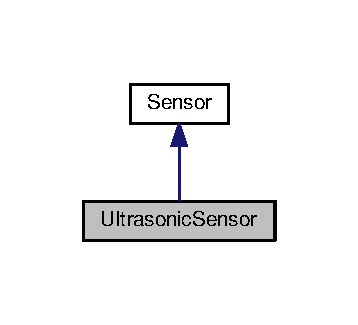
\includegraphics[width=172pt]{classUltrasonicSensor__inherit__graph}
\end{center}
\end{figure}


Collaboration diagram for Ultrasonic\-Sensor\-:
\nopagebreak
\begin{figure}[H]
\begin{center}
\leavevmode
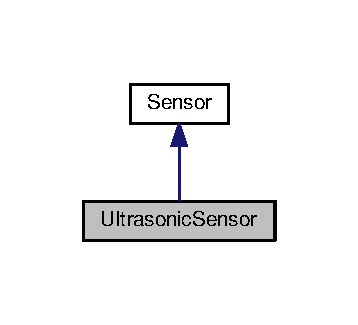
\includegraphics[width=172pt]{classUltrasonicSensor__coll__graph}
\end{center}
\end{figure}
\subsection*{Public Member Functions}
\begin{DoxyCompactItemize}
\item 
\hyperlink{classUltrasonicSensor_afc21cb39ba75dfd008e1e82c82d2e61f}{Ultrasonic\-Sensor} ()
\begin{DoxyCompactList}\small\item\em Class Constructor. \end{DoxyCompactList}\item 
virtual void \hyperlink{classUltrasonicSensor_aa825f00c93ee05ca0edbeb3a99f485b6}{set\-Maximum\-Range} (int max\-Range)
\begin{DoxyCompactList}\small\item\em Sets the maximum range of the Ultrasonic \hyperlink{classSensor}{Sensor}. \end{DoxyCompactList}\item 
virtual void \hyperlink{classUltrasonicSensor_a20010d13123da9fbf3efcdeb59d9f6a4}{set\-Gain} (int gain)
\begin{DoxyCompactList}\small\item\em Sets the gain of the Ultrasonic \hyperlink{classSensor}{Sensor}. \end{DoxyCompactList}\item 
virtual void \hyperlink{classUltrasonicSensor_a7e35552a5e39f38202c2a8650a90f43c}{init\-Driver} (int number\-Of\-Sensors, int gain, int max\-Range)
\begin{DoxyCompactList}\small\item\em Initiates Ultrasonic \hyperlink{classSensor}{Sensor} Driver. \end{DoxyCompactList}\item 
virtual std\-::vector$<$ int $>$ \hyperlink{classUltrasonicSensor_a4dab101931d788a031fe44db24d0c305}{get\-Sensor\-Data} ()
\begin{DoxyCompactList}\small\item\em Retrieves the Ultrasonic \hyperlink{classSensor}{Sensor} data. \end{DoxyCompactList}\item 
virtual void \hyperlink{classUltrasonicSensor_a5587d9432d42a82d9f6f853b0aecddd3}{generate\-Sensor\-Data} ()
\begin{DoxyCompactList}\small\item\em Generates the Ultrasonic \hyperlink{classSensor}{Sensor} data. \end{DoxyCompactList}\item 
virtual void \hyperlink{classUltrasonicSensor_ac24cc66755a3201fc667e43d7d0a62c5}{parse\-Sensor\-Data} (std\-::vector$<$ int $>$ data)
\begin{DoxyCompactList}\small\item\em Parses the Ultrasonic \hyperlink{classSensor}{Sensor} data vector into individual variables. \end{DoxyCompactList}\item 
virtual void \hyperlink{classUltrasonicSensor_a0f3de9fee2a0ff99f5163b778ecfad4d}{set\-Sensor\-Type} ()
\begin{DoxyCompactList}\small\item\em Sets the \hyperlink{classSensor}{Sensor} type as Ultrasonic. \end{DoxyCompactList}\item 
virtual std\-::string \hyperlink{classUltrasonicSensor_ac354871be24914dfbfad3f07af061403}{get\-Sensor\-Type} ()
\begin{DoxyCompactList}\small\item\em Retrieves the \hyperlink{classSensor}{Sensor} type\-: Ultrasonic. \end{DoxyCompactList}\item 
virtual void \hyperlink{classUltrasonicSensor_adbd980ad9471ccf285dede0c4a4c4def}{set\-Number\-Of\-Sensors} (int number)
\begin{DoxyCompactList}\small\item\em Configures the number of ultrasonic sensors to be used (4) \end{DoxyCompactList}\item 
virtual void \hyperlink{classUltrasonicSensor_a9c92da2614f15035c069c7ae9ae2899d}{set\-Sensor\-Device\-I\-D} (int number\-Of\-Devices)
\begin{DoxyCompactList}\small\item\em Sets the device I\-Ds of the ultrasonic sensors. \end{DoxyCompactList}\item 
virtual void \hyperlink{classUltrasonicSensor_a1676043861eb34cb61e27002212b90cc}{get\-Sensor\-Device\-I\-D} ()
\begin{DoxyCompactList}\small\item\em Prints to the screen the device I\-Ds of the ultrasonic sensors. \end{DoxyCompactList}\item 
virtual void \hyperlink{classUltrasonicSensor_ac101ee85a4d58f5bf075e18ece5776da}{get\-Time\-Stamp} ()
\begin{DoxyCompactList}\small\item\em Prints to the screen the ultrasonic sensor readings time stamp. \end{DoxyCompactList}\end{DoxyCompactItemize}


\subsection{Constructor \& Destructor Documentation}
\hypertarget{classUltrasonicSensor_afc21cb39ba75dfd008e1e82c82d2e61f}{\index{Ultrasonic\-Sensor@{Ultrasonic\-Sensor}!Ultrasonic\-Sensor@{Ultrasonic\-Sensor}}
\index{Ultrasonic\-Sensor@{Ultrasonic\-Sensor}!UltrasonicSensor@{Ultrasonic\-Sensor}}
\subsubsection[{Ultrasonic\-Sensor}]{\setlength{\rightskip}{0pt plus 5cm}Ultrasonic\-Sensor\-::\-Ultrasonic\-Sensor (
\begin{DoxyParamCaption}
{}
\end{DoxyParamCaption}
)}}\label{classUltrasonicSensor_afc21cb39ba75dfd008e1e82c82d2e61f}


Class Constructor. 


\begin{DoxyCode}
10                                    \{
11   sensorGain = 0;
12   sensorMaximumRange = 0;
13   numberOfSensors = 0;
14   ultrasonicSensorFront = 0;
15   ultrasonicSensorBack = 0;
16   ultrasonicSensorLeft = 0;
17   ultrasonicSensorRight = 0;
18 \}
\end{DoxyCode}


\subsection{Member Function Documentation}
\hypertarget{classUltrasonicSensor_a5587d9432d42a82d9f6f853b0aecddd3}{\index{Ultrasonic\-Sensor@{Ultrasonic\-Sensor}!generate\-Sensor\-Data@{generate\-Sensor\-Data}}
\index{generate\-Sensor\-Data@{generate\-Sensor\-Data}!UltrasonicSensor@{Ultrasonic\-Sensor}}
\subsubsection[{generate\-Sensor\-Data}]{\setlength{\rightskip}{0pt plus 5cm}void Ultrasonic\-Sensor\-::generate\-Sensor\-Data (
\begin{DoxyParamCaption}
{}
\end{DoxyParamCaption}
)\hspace{0.3cm}{\ttfamily [virtual]}}}\label{classUltrasonicSensor_a5587d9432d42a82d9f6f853b0aecddd3}


Generates the Ultrasonic \hyperlink{classSensor}{Sensor} data. 


\begin{DoxyParams}{Parameters}
{\em none} & \\
\hline
\end{DoxyParams}
\begin{DoxyReturn}{Returns}
void function does not return anything 
\end{DoxyReturn}


Implements \hyperlink{classSensor_a1cabdc10d3319abeaa8db56724fa36e5}{Sensor}.


\begin{DoxyCode}
53                                           \{
54   std::random\_device rnd;
55   std::mt19937 gen(rnd());
56   std::uniform\_int\_distribution<> dist(1,100);
57   \textcolor{keywordflow}{for}(\textcolor{keyword}{auto} i=0;i<numberOfSensors;i++)
58     sensorData.push\_back(dist(gen));
59   \textcolor{keywordflow}{for}(\textcolor{keyword}{auto} n:sensorData)
60     std::cout << \hyperlink{classUltrasonicSensor_ac354871be24914dfbfad3f07af061403}{UltrasonicSensor::getSensorType}() <<\textcolor{stringliteral}{" Sensor = "} << n << 
      std::endl;
61 \}
\end{DoxyCode}
\hypertarget{classUltrasonicSensor_a4dab101931d788a031fe44db24d0c305}{\index{Ultrasonic\-Sensor@{Ultrasonic\-Sensor}!get\-Sensor\-Data@{get\-Sensor\-Data}}
\index{get\-Sensor\-Data@{get\-Sensor\-Data}!UltrasonicSensor@{Ultrasonic\-Sensor}}
\subsubsection[{get\-Sensor\-Data}]{\setlength{\rightskip}{0pt plus 5cm}std\-::vector$<$ int $>$ Ultrasonic\-Sensor\-::get\-Sensor\-Data (
\begin{DoxyParamCaption}
{}
\end{DoxyParamCaption}
)\hspace{0.3cm}{\ttfamily [virtual]}}}\label{classUltrasonicSensor_a4dab101931d788a031fe44db24d0c305}


Retrieves the Ultrasonic \hyperlink{classSensor}{Sensor} data. 


\begin{DoxyParams}{Parameters}
{\em none} & \\
\hline
\end{DoxyParams}
\begin{DoxyReturn}{Returns}
vector$<$int$>$ vector containing 4 sensor readings 
\end{DoxyReturn}


Implements \hyperlink{classSensor_a795dda4f99ae87b9d66c3c5a07722d1b}{Sensor}.


\begin{DoxyCode}
49                                                \{
50   \textcolor{keywordflow}{return} sensorData;
51 \}
\end{DoxyCode}
\hypertarget{classUltrasonicSensor_a1676043861eb34cb61e27002212b90cc}{\index{Ultrasonic\-Sensor@{Ultrasonic\-Sensor}!get\-Sensor\-Device\-I\-D@{get\-Sensor\-Device\-I\-D}}
\index{get\-Sensor\-Device\-I\-D@{get\-Sensor\-Device\-I\-D}!UltrasonicSensor@{Ultrasonic\-Sensor}}
\subsubsection[{get\-Sensor\-Device\-I\-D}]{\setlength{\rightskip}{0pt plus 5cm}void Ultrasonic\-Sensor\-::get\-Sensor\-Device\-I\-D (
\begin{DoxyParamCaption}
{}
\end{DoxyParamCaption}
)\hspace{0.3cm}{\ttfamily [virtual]}}}\label{classUltrasonicSensor_a1676043861eb34cb61e27002212b90cc}


Prints to the screen the device I\-Ds of the ultrasonic sensors. 


\begin{DoxyParams}{Parameters}
{\em none} & \\
\hline
\end{DoxyParams}
\begin{DoxyReturn}{Returns}
void function does not return anything 
\end{DoxyReturn}


Implements \hyperlink{classSensor_af7ff987e1f0f6b7c4acf2910212fde95}{Sensor}.


\begin{DoxyCode}
95                                          \{
96   std::cout <<\textcolor{stringliteral}{"Sensor Front device ID : "} << deviceID.at(0) << std::endl;
97   std::cout <<\textcolor{stringliteral}{"Sensor Back  device ID : "} << deviceID.at(1) << std::endl;
98   std::cout <<\textcolor{stringliteral}{"Sensor Left  device ID : "} << deviceID.at(2) << std::endl;
99   std::cout <<\textcolor{stringliteral}{"Sensor Right device ID : "} << deviceID.at(3) << std::endl;
100 \}
\end{DoxyCode}
\hypertarget{classUltrasonicSensor_ac354871be24914dfbfad3f07af061403}{\index{Ultrasonic\-Sensor@{Ultrasonic\-Sensor}!get\-Sensor\-Type@{get\-Sensor\-Type}}
\index{get\-Sensor\-Type@{get\-Sensor\-Type}!UltrasonicSensor@{Ultrasonic\-Sensor}}
\subsubsection[{get\-Sensor\-Type}]{\setlength{\rightskip}{0pt plus 5cm}std\-::string Ultrasonic\-Sensor\-::get\-Sensor\-Type (
\begin{DoxyParamCaption}
{}
\end{DoxyParamCaption}
)\hspace{0.3cm}{\ttfamily [virtual]}}}\label{classUltrasonicSensor_ac354871be24914dfbfad3f07af061403}


Retrieves the \hyperlink{classSensor}{Sensor} type\-: Ultrasonic. 


\begin{DoxyParams}{Parameters}
{\em none} & \\
\hline
\end{DoxyParams}
\begin{DoxyReturn}{Returns}
string Contains the sensor type (ultrasonic) 
\end{DoxyReturn}


Implements \hyperlink{classSensor_a6cf36c37e69761711982fed5d14aeb4e}{Sensor}.


\begin{DoxyCode}
78                                           \{
79   \textcolor{keywordflow}{return} sensorType;
80 \}
\end{DoxyCode}
\hypertarget{classUltrasonicSensor_ac101ee85a4d58f5bf075e18ece5776da}{\index{Ultrasonic\-Sensor@{Ultrasonic\-Sensor}!get\-Time\-Stamp@{get\-Time\-Stamp}}
\index{get\-Time\-Stamp@{get\-Time\-Stamp}!UltrasonicSensor@{Ultrasonic\-Sensor}}
\subsubsection[{get\-Time\-Stamp}]{\setlength{\rightskip}{0pt plus 5cm}void Ultrasonic\-Sensor\-::get\-Time\-Stamp (
\begin{DoxyParamCaption}
{}
\end{DoxyParamCaption}
)\hspace{0.3cm}{\ttfamily [virtual]}}}\label{classUltrasonicSensor_ac101ee85a4d58f5bf075e18ece5776da}


Prints to the screen the ultrasonic sensor readings time stamp. 


\begin{DoxyParams}{Parameters}
{\em none} & \\
\hline
\end{DoxyParams}
\begin{DoxyReturn}{Returns}
void function does not return anything 
\end{DoxyReturn}


Implements \hyperlink{classSensor_a8c6ceb519eb8720a0e9cedd84624a7ff}{Sensor}.


\begin{DoxyCode}
102                                     \{
103   \textcolor{keyword}{auto} now = std::chrono::system\_clock::now();
104   \textcolor{keyword}{auto} nowC = std::chrono::system\_clock::to\_time\_t(now);
105   std::cout << \textcolor{stringliteral}{"Time stamp = "} << std::ctime(&nowC) << std::endl;
106 \}
\end{DoxyCode}
\hypertarget{classUltrasonicSensor_a7e35552a5e39f38202c2a8650a90f43c}{\index{Ultrasonic\-Sensor@{Ultrasonic\-Sensor}!init\-Driver@{init\-Driver}}
\index{init\-Driver@{init\-Driver}!UltrasonicSensor@{Ultrasonic\-Sensor}}
\subsubsection[{init\-Driver}]{\setlength{\rightskip}{0pt plus 5cm}void Ultrasonic\-Sensor\-::init\-Driver (
\begin{DoxyParamCaption}
\item[{int}]{number\-Of\-Sensors, }
\item[{int}]{gain, }
\item[{int}]{max\-Range}
\end{DoxyParamCaption}
)\hspace{0.3cm}{\ttfamily [virtual]}}}\label{classUltrasonicSensor_a7e35552a5e39f38202c2a8650a90f43c}


Initiates Ultrasonic \hyperlink{classSensor}{Sensor} Driver. 


\begin{DoxyParams}{Parameters}
{\em number\-Of\-Sensors} & sets the number of sensors in the module \\
\hline
{\em gain} & sets the gain of the module \\
\hline
{\em max\-Range} & sets the maximum range of the module \\
\hline
\end{DoxyParams}
\begin{DoxyReturn}{Returns}
void function does not return anything
\end{DoxyReturn}
This method executes all initialization functions for the module. 

Implements \hyperlink{classSensor_a12851eb9413ee61c2d694b4168e365fd}{Sensor}.


\begin{DoxyCode}
20                                                                             \{
21   \textcolor{keywordflow}{if} (std::isless(numberOfSensors,0) || std::isless(gain,0) || std::isless(maxRange,0))
22     \textcolor{keywordflow}{throw} std::domain\_error(\textcolor{stringliteral}{"Negative arguments are invalid"});
23   std::cout <<\textcolor{stringliteral}{"=====================================\(\backslash\)n"};
24   std::cout <<\textcolor{stringliteral}{"Initializing Ultrasonic Sensors.....!\(\backslash\)n"};
25   std::cout <<\textcolor{stringliteral}{".....................................\(\backslash\)n"};
26   \hyperlink{classUltrasonicSensor_a0f3de9fee2a0ff99f5163b778ecfad4d}{UltrasonicSensor::setSensorType}();
27   \hyperlink{classUltrasonicSensor_a20010d13123da9fbf3efcdeb59d9f6a4}{UltrasonicSensor::setGain}(gain);
28   \hyperlink{classUltrasonicSensor_aa825f00c93ee05ca0edbeb3a99f485b6}{UltrasonicSensor::setMaximumRange}(maxRange);
29   \hyperlink{classUltrasonicSensor_a9c92da2614f15035c069c7ae9ae2899d}{UltrasonicSensor::setSensorDeviceID}(numberOfSensors);
30   \hyperlink{classUltrasonicSensor_adbd980ad9471ccf285dede0c4a4c4def}{UltrasonicSensor::setNumberOfSensors}(numberOfSensors);
31   \hyperlink{classUltrasonicSensor_a1676043861eb34cb61e27002212b90cc}{UltrasonicSensor::getSensorDeviceID}();
32   std::cout <<\textcolor{stringliteral}{".....................................\(\backslash\)n"};
33 \}
\end{DoxyCode}
\hypertarget{classUltrasonicSensor_ac24cc66755a3201fc667e43d7d0a62c5}{\index{Ultrasonic\-Sensor@{Ultrasonic\-Sensor}!parse\-Sensor\-Data@{parse\-Sensor\-Data}}
\index{parse\-Sensor\-Data@{parse\-Sensor\-Data}!UltrasonicSensor@{Ultrasonic\-Sensor}}
\subsubsection[{parse\-Sensor\-Data}]{\setlength{\rightskip}{0pt plus 5cm}void Ultrasonic\-Sensor\-::parse\-Sensor\-Data (
\begin{DoxyParamCaption}
\item[{std\-::vector$<$ int $>$}]{data}
\end{DoxyParamCaption}
)\hspace{0.3cm}{\ttfamily [virtual]}}}\label{classUltrasonicSensor_ac24cc66755a3201fc667e43d7d0a62c5}


Parses the Ultrasonic \hyperlink{classSensor}{Sensor} data vector into individual variables. 


\begin{DoxyParams}{Parameters}
{\em data} & vector containing 4 integer readings \\
\hline
\end{DoxyParams}
\begin{DoxyReturn}{Returns}
void function does not return anything 
\end{DoxyReturn}


Implements \hyperlink{classSensor_a32f0d1754f66bdb26bbece93e05b9a44}{Sensor}.


\begin{DoxyCode}
62                                                           \{
63   ultrasonicSensorFront = data.at(0);
64   std::cout <<\textcolor{stringliteral}{"Sensor Front value = "} << ultrasonicSensorFront << std::endl;
65   ultrasonicSensorBack  = data.at(1);
66   std::cout <<\textcolor{stringliteral}{"Sensor Back value = "} << ultrasonicSensorBack << std::endl;  
67   ultrasonicSensorLeft  = data.at(2);
68   std::cout <<\textcolor{stringliteral}{"Sensor Left value = "} << ultrasonicSensorLeft << std::endl;
69   ultrasonicSensorRight = data.at(3);
70   std::cout <<\textcolor{stringliteral}{"Sensor Right value = "} << ultrasonicSensorRight << std::endl;
71 \}
\end{DoxyCode}
\hypertarget{classUltrasonicSensor_a20010d13123da9fbf3efcdeb59d9f6a4}{\index{Ultrasonic\-Sensor@{Ultrasonic\-Sensor}!set\-Gain@{set\-Gain}}
\index{set\-Gain@{set\-Gain}!UltrasonicSensor@{Ultrasonic\-Sensor}}
\subsubsection[{set\-Gain}]{\setlength{\rightskip}{0pt plus 5cm}void Ultrasonic\-Sensor\-::set\-Gain (
\begin{DoxyParamCaption}
\item[{int}]{gain}
\end{DoxyParamCaption}
)\hspace{0.3cm}{\ttfamily [virtual]}}}\label{classUltrasonicSensor_a20010d13123da9fbf3efcdeb59d9f6a4}


Sets the gain of the Ultrasonic \hyperlink{classSensor}{Sensor}. 


\begin{DoxyParams}{Parameters}
{\em gain} & sensor gain \\
\hline
\end{DoxyParams}
\begin{DoxyReturn}{Returns}
void function does not return anything 
\end{DoxyReturn}

\begin{DoxyCode}
42                                        \{
43   \textcolor{keywordflow}{if} (std::isless(gain,0))
44     \textcolor{keywordflow}{throw} std::domain\_error(\textcolor{stringliteral}{"Negative gain not allowed"});
45   sensorGain = gain;
46   std::cout <<\textcolor{stringliteral}{"Sensor gain : "} << sensorGain << std::endl;
47 \}
\end{DoxyCode}
\hypertarget{classUltrasonicSensor_aa825f00c93ee05ca0edbeb3a99f485b6}{\index{Ultrasonic\-Sensor@{Ultrasonic\-Sensor}!set\-Maximum\-Range@{set\-Maximum\-Range}}
\index{set\-Maximum\-Range@{set\-Maximum\-Range}!UltrasonicSensor@{Ultrasonic\-Sensor}}
\subsubsection[{set\-Maximum\-Range}]{\setlength{\rightskip}{0pt plus 5cm}void Ultrasonic\-Sensor\-::set\-Maximum\-Range (
\begin{DoxyParamCaption}
\item[{int}]{max\-Range}
\end{DoxyParamCaption}
)\hspace{0.3cm}{\ttfamily [virtual]}}}\label{classUltrasonicSensor_aa825f00c93ee05ca0edbeb3a99f485b6}


Sets the maximum range of the Ultrasonic \hyperlink{classSensor}{Sensor}. 


\begin{DoxyParams}{Parameters}
{\em max\-Range} & maximum range \\
\hline
\end{DoxyParams}
\begin{DoxyReturn}{Returns}
void function does not return anything 
\end{DoxyReturn}

\begin{DoxyCode}
35                                                    \{
36   \textcolor{keywordflow}{if} (std::isless(maxRange,0))
37     \textcolor{keywordflow}{throw} std::domain\_error(\textcolor{stringliteral}{"Negative range not allowed"});
38   sensorMaximumRange = maxRange;
39   std::cout <<\textcolor{stringliteral}{"Sensor Maximum range : "} << sensorMaximumRange << std::endl;
40 \}
\end{DoxyCode}
\hypertarget{classUltrasonicSensor_adbd980ad9471ccf285dede0c4a4c4def}{\index{Ultrasonic\-Sensor@{Ultrasonic\-Sensor}!set\-Number\-Of\-Sensors@{set\-Number\-Of\-Sensors}}
\index{set\-Number\-Of\-Sensors@{set\-Number\-Of\-Sensors}!UltrasonicSensor@{Ultrasonic\-Sensor}}
\subsubsection[{set\-Number\-Of\-Sensors}]{\setlength{\rightskip}{0pt plus 5cm}void Ultrasonic\-Sensor\-::set\-Number\-Of\-Sensors (
\begin{DoxyParamCaption}
\item[{int}]{number}
\end{DoxyParamCaption}
)\hspace{0.3cm}{\ttfamily [virtual]}}}\label{classUltrasonicSensor_adbd980ad9471ccf285dede0c4a4c4def}


Configures the number of ultrasonic sensors to be used (4) 


\begin{DoxyParams}{Parameters}
{\em number} & number of sensors \\
\hline
\end{DoxyParams}
\begin{DoxyReturn}{Returns}
void function does not return anything 
\end{DoxyReturn}


Implements \hyperlink{classSensor_a5372c229e1bf77d70d48506af8abd351}{Sensor}.


\begin{DoxyCode}
82                                                     \{
83   \textcolor{keywordflow}{if} (std::isless(number,0))
84     \textcolor{keywordflow}{throw} std::domain\_error(\textcolor{stringliteral}{"Negative arguments are invalid"});
85   numberOfSensors = number;
86 \}
\end{DoxyCode}
\hypertarget{classUltrasonicSensor_a9c92da2614f15035c069c7ae9ae2899d}{\index{Ultrasonic\-Sensor@{Ultrasonic\-Sensor}!set\-Sensor\-Device\-I\-D@{set\-Sensor\-Device\-I\-D}}
\index{set\-Sensor\-Device\-I\-D@{set\-Sensor\-Device\-I\-D}!UltrasonicSensor@{Ultrasonic\-Sensor}}
\subsubsection[{set\-Sensor\-Device\-I\-D}]{\setlength{\rightskip}{0pt plus 5cm}void Ultrasonic\-Sensor\-::set\-Sensor\-Device\-I\-D (
\begin{DoxyParamCaption}
\item[{int}]{number\-Of\-Devices}
\end{DoxyParamCaption}
)\hspace{0.3cm}{\ttfamily [virtual]}}}\label{classUltrasonicSensor_a9c92da2614f15035c069c7ae9ae2899d}


Sets the device I\-Ds of the ultrasonic sensors. 


\begin{DoxyParams}{Parameters}
{\em number\-Of\-Devices} & number of devices \\
\hline
\end{DoxyParams}
\begin{DoxyReturn}{Returns}
void function does not return anything 
\end{DoxyReturn}


Implements \hyperlink{classSensor_a3a7ad3cdc0e9a5ef6f5ce684c7a0c59a}{Sensor}.


\begin{DoxyCode}
88                                                             \{
89   \textcolor{keywordflow}{if} (std::isless(numberOfDevices,0))
90     \textcolor{keywordflow}{throw} std::domain\_error(\textcolor{stringliteral}{"Negative arguments are invalid"});
91   \textcolor{keywordflow}{for} (\textcolor{keyword}{auto} i =1; i <= numberOfDevices; i++)
92     deviceID.push\_back(i*10);
93 \}
\end{DoxyCode}
\hypertarget{classUltrasonicSensor_a0f3de9fee2a0ff99f5163b778ecfad4d}{\index{Ultrasonic\-Sensor@{Ultrasonic\-Sensor}!set\-Sensor\-Type@{set\-Sensor\-Type}}
\index{set\-Sensor\-Type@{set\-Sensor\-Type}!UltrasonicSensor@{Ultrasonic\-Sensor}}
\subsubsection[{set\-Sensor\-Type}]{\setlength{\rightskip}{0pt plus 5cm}void Ultrasonic\-Sensor\-::set\-Sensor\-Type (
\begin{DoxyParamCaption}
{}
\end{DoxyParamCaption}
)\hspace{0.3cm}{\ttfamily [virtual]}}}\label{classUltrasonicSensor_a0f3de9fee2a0ff99f5163b778ecfad4d}


Sets the \hyperlink{classSensor}{Sensor} type as Ultrasonic. 


\begin{DoxyParams}{Parameters}
{\em none} & \\
\hline
\end{DoxyParams}
\begin{DoxyReturn}{Returns}
void function does not return anything 
\end{DoxyReturn}


Implements \hyperlink{classSensor_a53daf1760d09355a8d3846addc53bd6e}{Sensor}.


\begin{DoxyCode}
73                                      \{
74   sensorType = \textcolor{stringliteral}{"Ultrasonic"};
75   std::cout <<\textcolor{stringliteral}{"Sensor Type : "} << \hyperlink{classUltrasonicSensor_ac354871be24914dfbfad3f07af061403}{UltrasonicSensor::getSensorType}() << 
      std::endl;
76 \}
\end{DoxyCode}


The documentation for this class was generated from the following files\-:\begin{DoxyCompactItemize}
\item 
Obstacle\-Avoidance/include/\hyperlink{UltrasonicSensor_8h}{Ultrasonic\-Sensor.\-h}\item 
Obstacle\-Avoidance/app/\hyperlink{UltrasonicSensor_8cpp}{Ultrasonic\-Sensor.\-cpp}\end{DoxyCompactItemize}

\chapter{File Documentation}
\hypertarget{LaserSensor_8cpp}{\section{Obstacle\-Avoidance/app/\-Laser\-Sensor.cpp File Reference}
\label{LaserSensor_8cpp}\index{Obstacle\-Avoidance/app/\-Laser\-Sensor.\-cpp@{Obstacle\-Avoidance/app/\-Laser\-Sensor.\-cpp}}
}
{\ttfamily \#include \char`\"{}Laser\-Sensor.\-h\char`\"{}}\\*
Include dependency graph for Laser\-Sensor.\-cpp\-:
\nopagebreak
\begin{figure}[H]
\begin{center}
\leavevmode
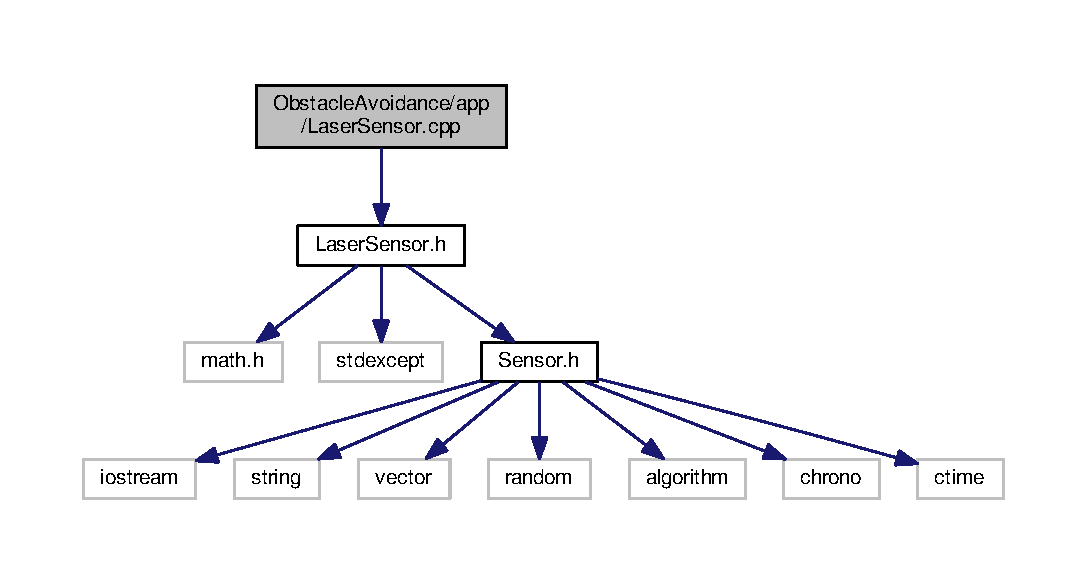
\includegraphics[width=350pt]{LaserSensor_8cpp__incl}
\end{center}
\end{figure}

\hypertarget{main_8cpp}{\section{Obstacle\-Avoidance/app/main.cpp File Reference}
\label{main_8cpp}\index{Obstacle\-Avoidance/app/main.\-cpp@{Obstacle\-Avoidance/app/main.\-cpp}}
}
{\ttfamily \#include \char`\"{}Ultrasonic\-Sensor.\-h\char`\"{}}\\*
{\ttfamily \#include \char`\"{}Laser\-Sensor.\-h\char`\"{}}\\*
{\ttfamily \#include \char`\"{}Sensor\-Fusion.\-h\char`\"{}}\\*
{\ttfamily \#include \char`\"{}Obstacle\-Avoidance\-Module.\-h\char`\"{}}\\*
{\ttfamily \#include \char`\"{}Motor\-Controller.\-h\char`\"{}}\\*
Include dependency graph for main.\-cpp\-:
\nopagebreak
\begin{figure}[H]
\begin{center}
\leavevmode
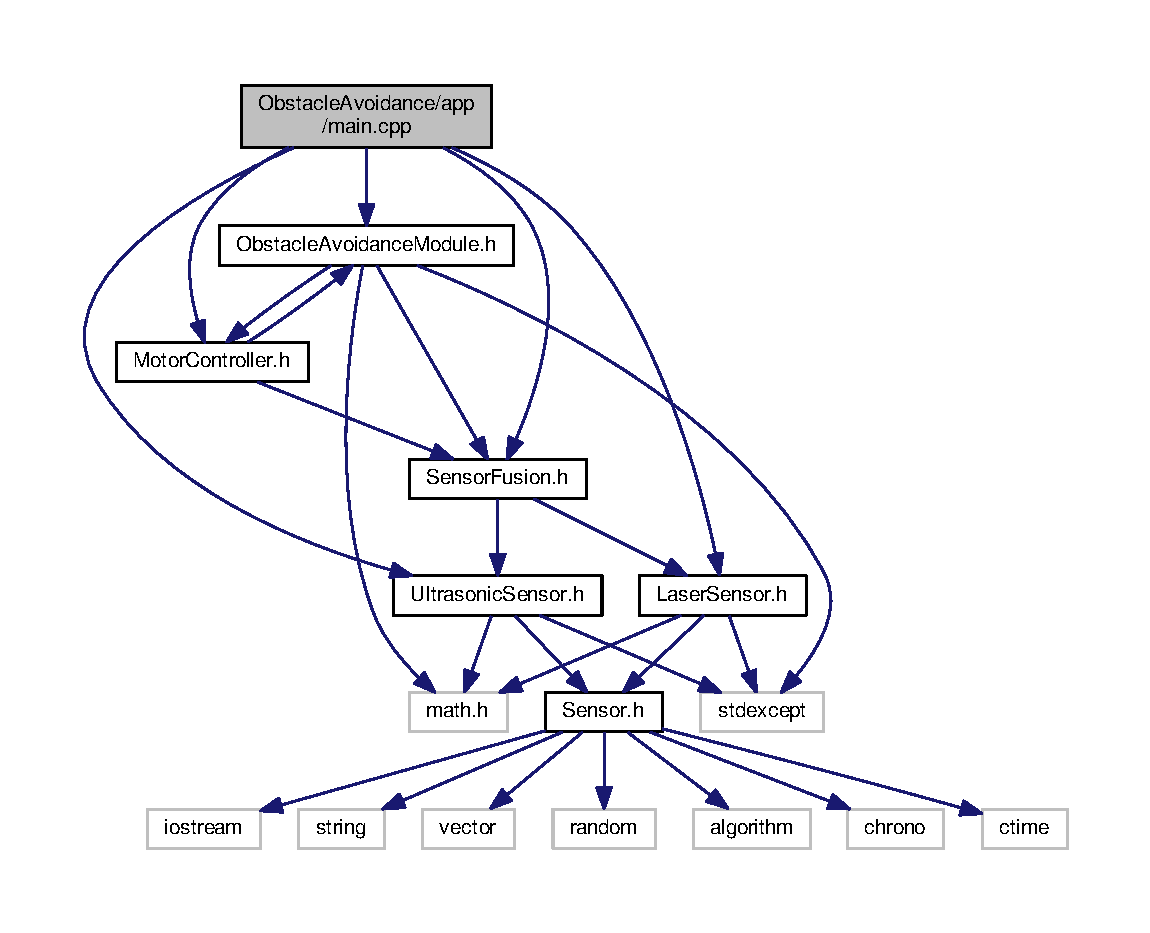
\includegraphics[width=350pt]{main_8cpp__incl}
\end{center}
\end{figure}
\subsection*{Functions}
\begin{DoxyCompactItemize}
\item 
int \hyperlink{main_8cpp_ae66f6b31b5ad750f1fe042a706a4e3d4}{main} ()
\end{DoxyCompactItemize}


\subsection{Function Documentation}
\hypertarget{main_8cpp_ae66f6b31b5ad750f1fe042a706a4e3d4}{\index{main.\-cpp@{main.\-cpp}!main@{main}}
\index{main@{main}!main.cpp@{main.\-cpp}}
\subsubsection[{main}]{\setlength{\rightskip}{0pt plus 5cm}int main (
\begin{DoxyParamCaption}
{}
\end{DoxyParamCaption}
)}}\label{main_8cpp_ae66f6b31b5ad750f1fe042a706a4e3d4}

\begin{DoxyCode}
14            \{
15   \hyperlink{classMotorController}{MotorController} mCtrl;
16   mCtrl.\hyperlink{classMotorController_a56ae5e4c44399b8afe94eb721514dd5e}{initializeMotorController}();
17   std::cout <<\textcolor{stringliteral}{"=====================================!\(\backslash\)n"};
18   std::cout <<\textcolor{stringliteral}{"Initialization Complete..............!\(\backslash\)n"};
19   std::cout <<\textcolor{stringliteral}{".....................................!\(\backslash\)n"};
20   std::cout <<\textcolor{stringliteral}{"Ready to drive.......................!\(\backslash\)n"};
21   \textcolor{keywordtype}{int} usrInFrontSpeed = 1;
22   mCtrl.\hyperlink{classMotorController_ab0dffd70556dbab55aa990673e6dc5f8}{moveForward}(usrInFrontSpeed);
23   \textcolor{keywordtype}{int} usrInLeftSpeed = 1;
24   mCtrl.\hyperlink{classMotorController_a4c3beafe5316cd08fd44845e20ec7151}{moveLeft}(usrInLeftSpeed);
25   \textcolor{keywordtype}{int} usrInBackSpeed = 1;
26   mCtrl.\hyperlink{classMotorController_a3ad21d7cff7b0c3c6700b2755b1df2d2}{moveBackwards}(usrInBackSpeed);
27   \textcolor{keywordtype}{int} usrInRightSpeed = 1;
28   mCtrl.\hyperlink{classMotorController_aa1586060f2ee0f66e83d30c897a1cdb4}{moveRight}(usrInRightSpeed);
29   std::cout <<\textcolor{stringliteral}{".....................................!\(\backslash\)n"};
30   std::cout <<\textcolor{stringliteral}{"Turning on Obstacle Avoidance Module.!\(\backslash\)n"};
31   std::cout <<\textcolor{stringliteral}{".....................................!\(\backslash\)n"};
32   \hyperlink{classUltrasonicSensor}{UltrasonicSensor} ultrSensor;
33   ultrSensor.\hyperlink{classUltrasonicSensor_a7e35552a5e39f38202c2a8650a90f43c}{initDriver}(4,10,100);
34   \hyperlink{classLaserSensor}{LaserSensor} lsrSensor;
35   lsrSensor.\hyperlink{classLaserSensor_a1137c622e564b5706e6f36e253c2828b}{initDriver}(4,15,150);
36   std::cout <<\textcolor{stringliteral}{"Reading Ultrasonic Sensor raw data...!\(\backslash\)n"};
37   ultrSensor.\hyperlink{classUltrasonicSensor_a5587d9432d42a82d9f6f853b0aecddd3}{generateSensorData}();
38   ultrSensor.\hyperlink{classUltrasonicSensor_ac101ee85a4d58f5bf075e18ece5776da}{getTimeStamp}();
39   std::cout <<\textcolor{stringliteral}{"Reading Laser Sensor raw data........!\(\backslash\)n"};
40   lsrSensor.\hyperlink{classLaserSensor_a87ed0b803f91e74752a9097c594bcb0a}{generateSensorData}();
41   lsrSensor.\hyperlink{classLaserSensor_a3be8d859cdab60a5e32c0855e5be928e}{getTimeStamp}();
42   std::cout <<\textcolor{stringliteral}{".....................................!\(\backslash\)n"};
43   std::cout <<\textcolor{stringliteral}{"Parsing Ultrasonic Sensors data......!\(\backslash\)n"};
44   ultrSensor.\hyperlink{classUltrasonicSensor_ac24cc66755a3201fc667e43d7d0a62c5}{parseSensorData}(ultrSensor.\hyperlink{classUltrasonicSensor_a4dab101931d788a031fe44db24d0c305}{getSensorData}());
45   std::cout <<\textcolor{stringliteral}{"Parsing Laser Sensors data...........!\(\backslash\)n"};   
46   lsrSensor.\hyperlink{classLaserSensor_aa2edc4c57398799497859ab9373e9aa5}{parseSensorData}(lsrSensor.\hyperlink{classLaserSensor_a1660841aa809bc22abc607780bf832b0}{getSensorData}());
47   std::cout <<\textcolor{stringliteral}{"Fusing Ultrasonic and Laser data.....!\(\backslash\)n"};
48   std::cout <<\textcolor{stringliteral}{".....................................!\(\backslash\)n"};
49   \hyperlink{classSensorFusion}{SensorFusion} fsdSensor;
50   fsdSensor.\hyperlink{classSensorFusion_a45b1154d5566e2a3368836b4aa5a3a4e}{fuseSensorData}(ultrSensor.\hyperlink{classUltrasonicSensor_a4dab101931d788a031fe44db24d0c305}{getSensorData}(), lsrSensor.
      \hyperlink{classLaserSensor_a1660841aa809bc22abc607780bf832b0}{getSensorData}());
51   fsdSensor.\hyperlink{classSensorFusion_a458c1aed280b12273476f0dd7f57f4c8}{outputFusedSensorData}();
52   std::cout <<\textcolor{stringliteral}{".....................................!\(\backslash\)n"};
53   \hyperlink{classObstacleAvoidance}{ObstacleAvoidance} obsAvMod;
54   obsAvMod.\hyperlink{classObstacleAvoidance_a05040b1d9096fa315e439a0a9cd3a0e3}{detectObstacle}(fsdSensor.\hyperlink{classSensorFusion_afc393d9d590acb884b37b720653d5ab5}{getFusedSensorFwd}(),fsdSensor.
      \hyperlink{classSensorFusion_aecba8be602ad5a5516c35ce2de0ef3cb}{getFusedSensorBack}(),fsdSensor.\hyperlink{classSensorFusion_a66d934da01cf106c27df5242e3e7394a}{getFusedSensorLeft}(),fsdSensor.
      \hyperlink{classSensorFusion_a4b408c81cc07c3b81d3bd34ad079715f}{getFusedSensorRight}());
55   obsAvMod.\hyperlink{classObstacleAvoidance_a646828a87a384074b80df0a0ff1320ec}{trnOnOffAvoid}(usrInFrontSpeed, usrInBackSpeed, usrInLeftSpeed, usrInRightSpeed);
56   mCtrl.\hyperlink{classMotorController_ab0dffd70556dbab55aa990673e6dc5f8}{moveForward}(usrInFrontSpeed);
57   mCtrl.\hyperlink{classMotorController_a4c3beafe5316cd08fd44845e20ec7151}{moveLeft}(usrInLeftSpeed);
58   mCtrl.\hyperlink{classMotorController_a3ad21d7cff7b0c3c6700b2755b1df2d2}{moveBackwards}(usrInBackSpeed);
59   mCtrl.\hyperlink{classMotorController_aa1586060f2ee0f66e83d30c897a1cdb4}{moveRight}(usrInRightSpeed);
60   \textcolor{keywordflow}{return} 0;
61 \}
\end{DoxyCode}

\hypertarget{MotorController_8cpp}{\section{Obstacle\-Avoidance/app/\-Motor\-Controller.cpp File Reference}
\label{MotorController_8cpp}\index{Obstacle\-Avoidance/app/\-Motor\-Controller.\-cpp@{Obstacle\-Avoidance/app/\-Motor\-Controller.\-cpp}}
}
{\ttfamily \#include \char`\"{}Motor\-Controller.\-h\char`\"{}}\\*
Include dependency graph for Motor\-Controller.\-cpp\-:
\nopagebreak
\begin{figure}[H]
\begin{center}
\leavevmode
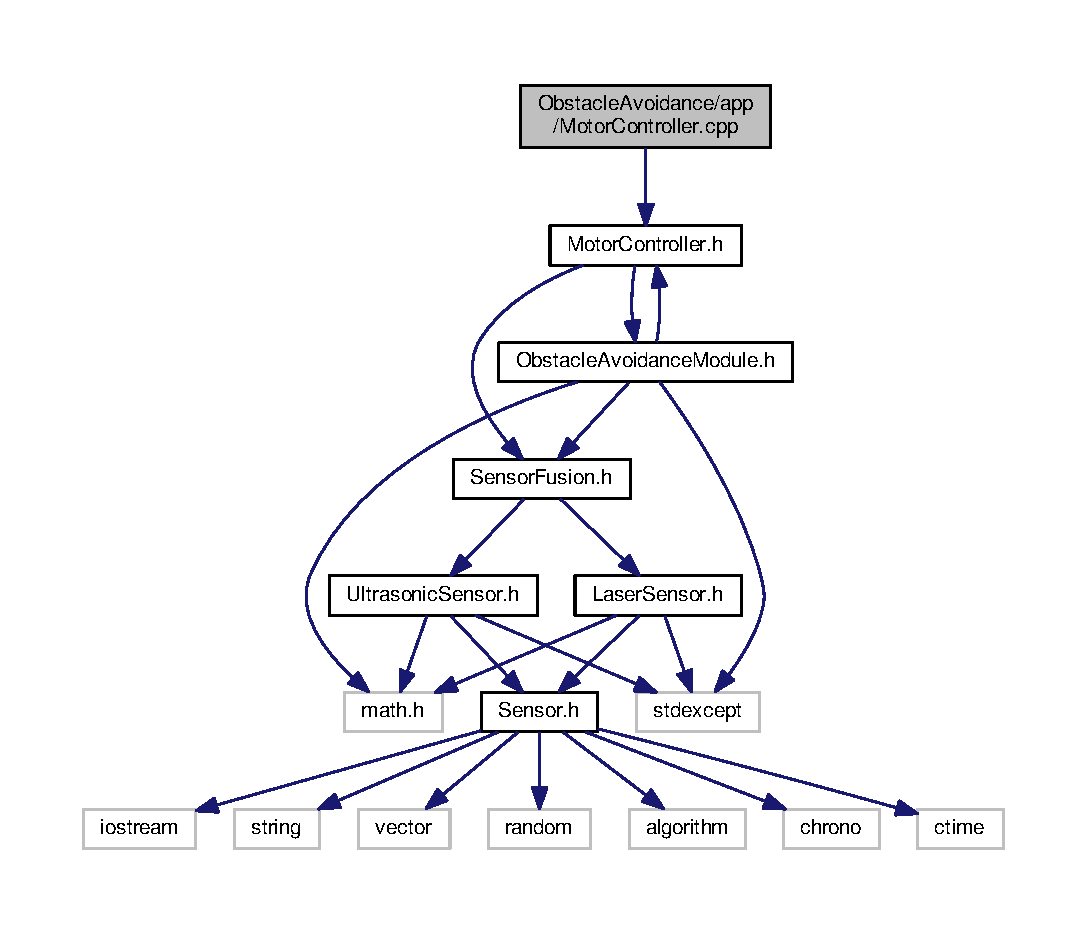
\includegraphics[width=350pt]{MotorController_8cpp__incl}
\end{center}
\end{figure}

\hypertarget{ObstacleAvoidanceModule_8cpp}{\section{Obstacle\-Avoidance/app/\-Obstacle\-Avoidance\-Module.cpp File Reference}
\label{ObstacleAvoidanceModule_8cpp}\index{Obstacle\-Avoidance/app/\-Obstacle\-Avoidance\-Module.\-cpp@{Obstacle\-Avoidance/app/\-Obstacle\-Avoidance\-Module.\-cpp}}
}
{\ttfamily \#include \char`\"{}Obstacle\-Avoidance\-Module.\-h\char`\"{}}\\*
Include dependency graph for Obstacle\-Avoidance\-Module.\-cpp\-:
\nopagebreak
\begin{figure}[H]
\begin{center}
\leavevmode
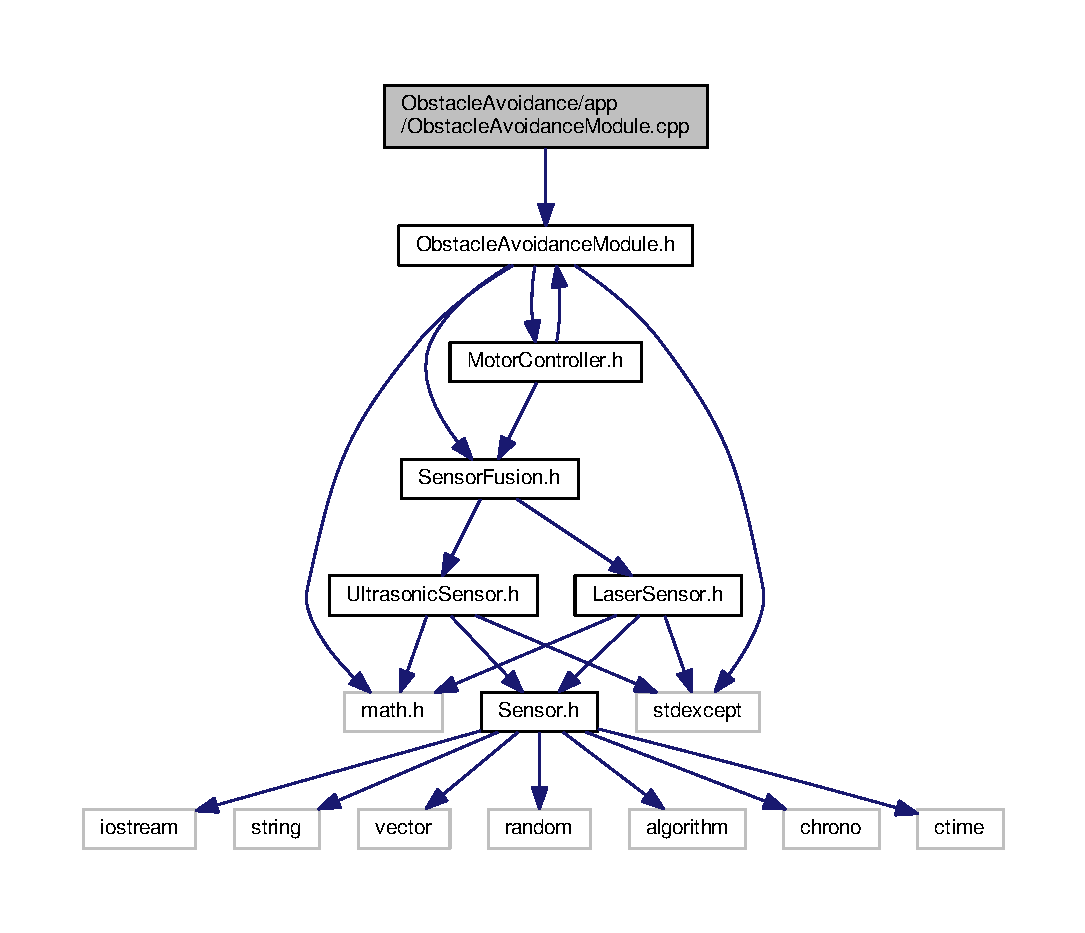
\includegraphics[width=350pt]{ObstacleAvoidanceModule_8cpp__incl}
\end{center}
\end{figure}

\hypertarget{SensorFusion_8cpp}{\section{Obstacle\-Avoidance/app/\-Sensor\-Fusion.cpp File Reference}
\label{SensorFusion_8cpp}\index{Obstacle\-Avoidance/app/\-Sensor\-Fusion.\-cpp@{Obstacle\-Avoidance/app/\-Sensor\-Fusion.\-cpp}}
}
{\ttfamily \#include \char`\"{}Sensor\-Fusion.\-h\char`\"{}}\\*
Include dependency graph for Sensor\-Fusion.\-cpp\-:
\nopagebreak
\begin{figure}[H]
\begin{center}
\leavevmode
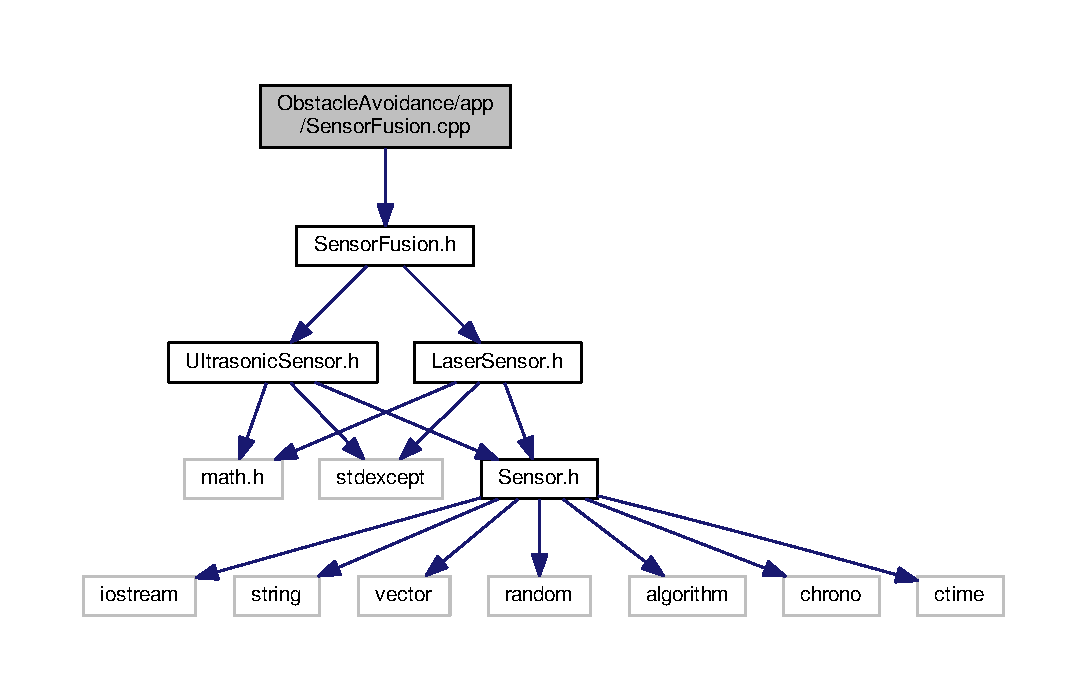
\includegraphics[width=350pt]{SensorFusion_8cpp__incl}
\end{center}
\end{figure}

\hypertarget{UltrasonicSensor_8cpp}{\section{Obstacle\-Avoidance/app/\-Ultrasonic\-Sensor.cpp File Reference}
\label{UltrasonicSensor_8cpp}\index{Obstacle\-Avoidance/app/\-Ultrasonic\-Sensor.\-cpp@{Obstacle\-Avoidance/app/\-Ultrasonic\-Sensor.\-cpp}}
}
{\ttfamily \#include \char`\"{}Ultrasonic\-Sensor.\-h\char`\"{}}\\*
Include dependency graph for Ultrasonic\-Sensor.\-cpp\-:
\nopagebreak
\begin{figure}[H]
\begin{center}
\leavevmode
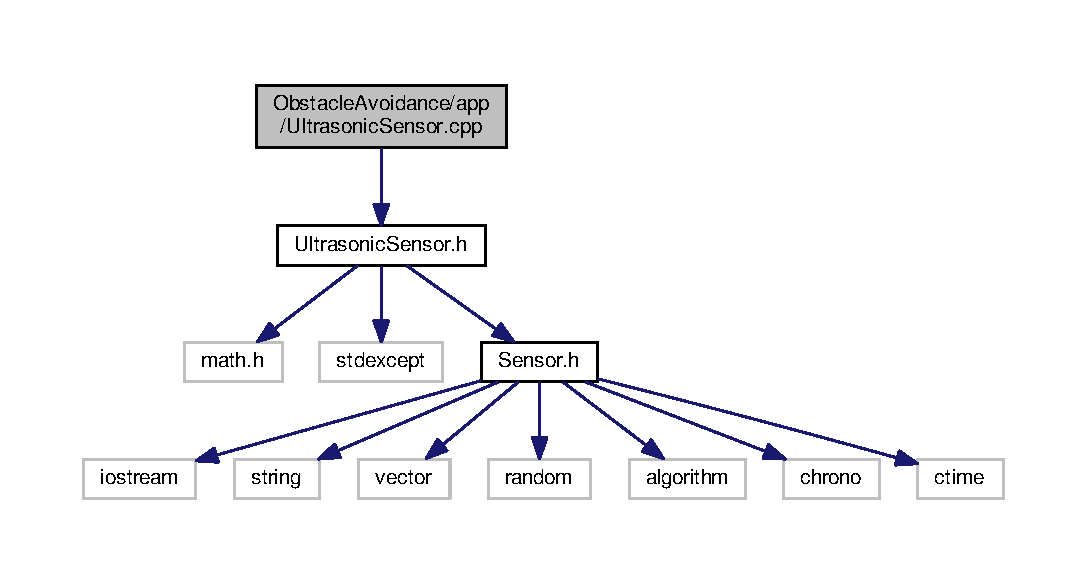
\includegraphics[width=350pt]{UltrasonicSensor_8cpp__incl}
\end{center}
\end{figure}

\hypertarget{LaserSensor_8h}{\section{Obstacle\-Avoidance/include/\-Laser\-Sensor.h File Reference}
\label{LaserSensor_8h}\index{Obstacle\-Avoidance/include/\-Laser\-Sensor.\-h@{Obstacle\-Avoidance/include/\-Laser\-Sensor.\-h}}
}


Simulates a laser sensor driver and generates laser sensor data.  


{\ttfamily \#include $<$math.\-h$>$}\\*
{\ttfamily \#include $<$stdexcept$>$}\\*
{\ttfamily \#include \char`\"{}Sensor.\-h\char`\"{}}\\*
Include dependency graph for Laser\-Sensor.\-h\-:
\nopagebreak
\begin{figure}[H]
\begin{center}
\leavevmode
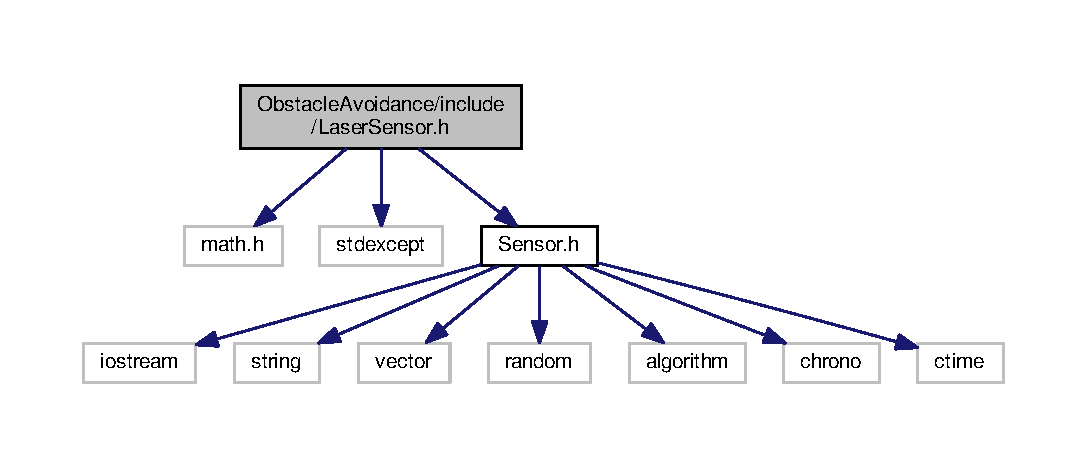
\includegraphics[width=350pt]{LaserSensor_8h__incl}
\end{center}
\end{figure}
This graph shows which files directly or indirectly include this file\-:
\nopagebreak
\begin{figure}[H]
\begin{center}
\leavevmode
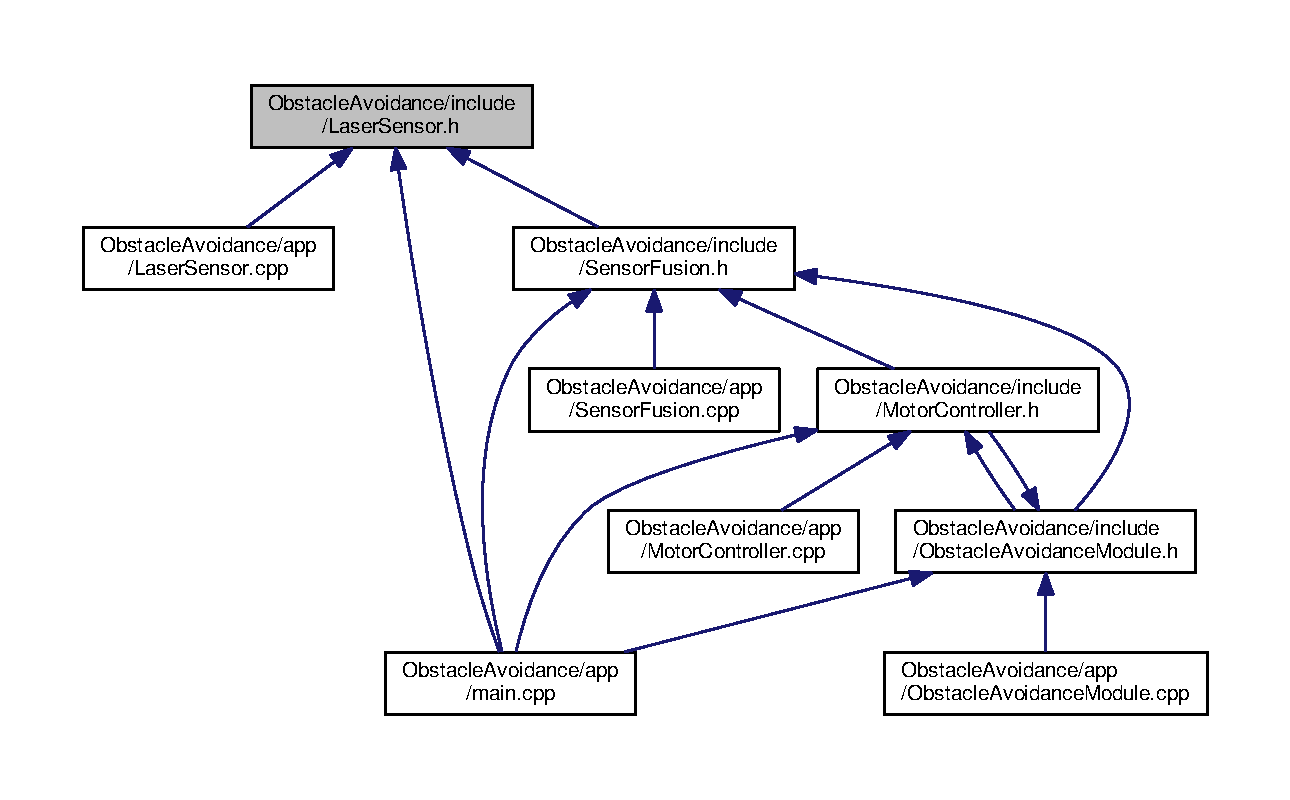
\includegraphics[width=350pt]{LaserSensor_8h__dep__incl}
\end{center}
\end{figure}
\subsection*{Classes}
\begin{DoxyCompactItemize}
\item 
class \hyperlink{classLaserSensor}{Laser\-Sensor}
\end{DoxyCompactItemize}


\subsection{Detailed Description}
Simulates a laser sensor driver and generates laser sensor data. Copyright 2017 Christian Ramos

\begin{DoxyVersion}{Version}
1.\-0 
\end{DoxyVersion}
\begin{DoxyDate}{Date}
Mar 7, 2017 
\end{DoxyDate}
\begin{DoxyAuthor}{Author}
Christian Ramos 
\end{DoxyAuthor}

\hypertarget{MotorController_8h}{\section{Obstacle\-Avoidance/include/\-Motor\-Controller.h File Reference}
\label{MotorController_8h}\index{Obstacle\-Avoidance/include/\-Motor\-Controller.\-h@{Obstacle\-Avoidance/include/\-Motor\-Controller.\-h}}
}


Simulates an omnidirectional vehicle Motor Controller driver that moves around at 1 to 2 mi/h.  


{\ttfamily \#include \char`\"{}Sensor\-Fusion.\-h\char`\"{}}\\*
{\ttfamily \#include \char`\"{}Obstacle\-Avoidance\-Module.\-h\char`\"{}}\\*
Include dependency graph for Motor\-Controller.\-h\-:
\nopagebreak
\begin{figure}[H]
\begin{center}
\leavevmode
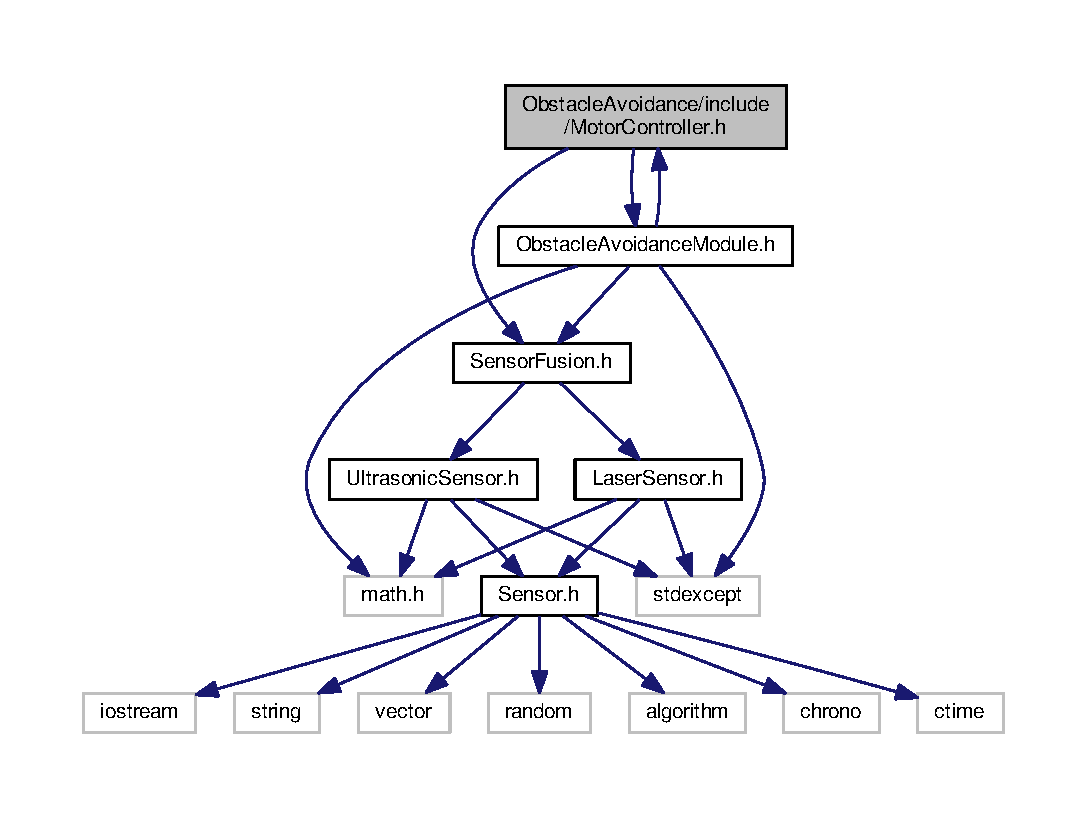
\includegraphics[width=350pt]{MotorController_8h__incl}
\end{center}
\end{figure}
This graph shows which files directly or indirectly include this file\-:
\nopagebreak
\begin{figure}[H]
\begin{center}
\leavevmode
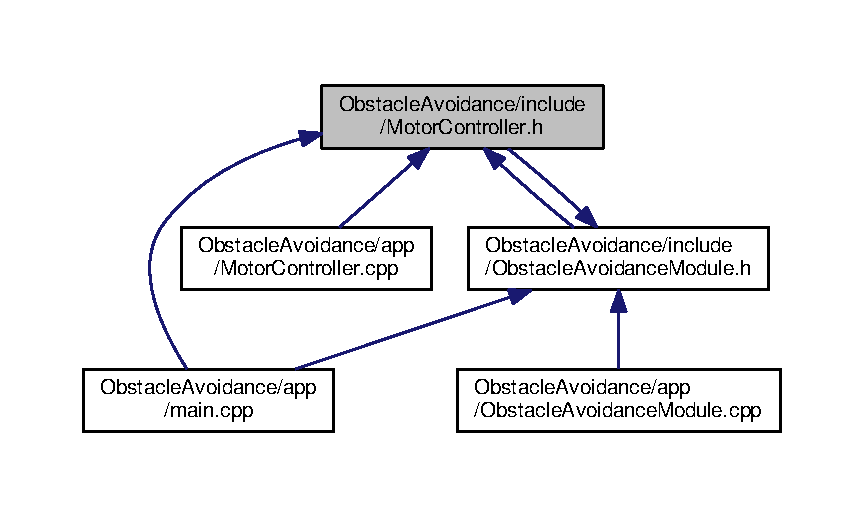
\includegraphics[width=350pt]{MotorController_8h__dep__incl}
\end{center}
\end{figure}
\subsection*{Classes}
\begin{DoxyCompactItemize}
\item 
class \hyperlink{classMotorController}{Motor\-Controller}
\end{DoxyCompactItemize}


\subsection{Detailed Description}
Simulates an omnidirectional vehicle Motor Controller driver that moves around at 1 to 2 mi/h. Copyright 2017 Christian Ramos

\begin{DoxyVersion}{Version}
1.\-0 
\end{DoxyVersion}
\begin{DoxyDate}{Date}
Mar 7, 2017 
\end{DoxyDate}
\begin{DoxyAuthor}{Author}
Christian Ramos 
\end{DoxyAuthor}

\hypertarget{ObstacleAvoidanceModule_8h}{\section{Obstacle\-Avoidance/include/\-Obstacle\-Avoidance\-Module.h File Reference}
\label{ObstacleAvoidanceModule_8h}\index{Obstacle\-Avoidance/include/\-Obstacle\-Avoidance\-Module.\-h@{Obstacle\-Avoidance/include/\-Obstacle\-Avoidance\-Module.\-h}}
}


Module that detects and avoids obstacles in the path of omnidirectional robotic vehicle.  


{\ttfamily \#include $<$math.\-h$>$}\\*
{\ttfamily \#include $<$stdexcept$>$}\\*
{\ttfamily \#include \char`\"{}Sensor\-Fusion.\-h\char`\"{}}\\*
{\ttfamily \#include \char`\"{}Motor\-Controller.\-h\char`\"{}}\\*
Include dependency graph for Obstacle\-Avoidance\-Module.\-h\-:
\nopagebreak
\begin{figure}[H]
\begin{center}
\leavevmode
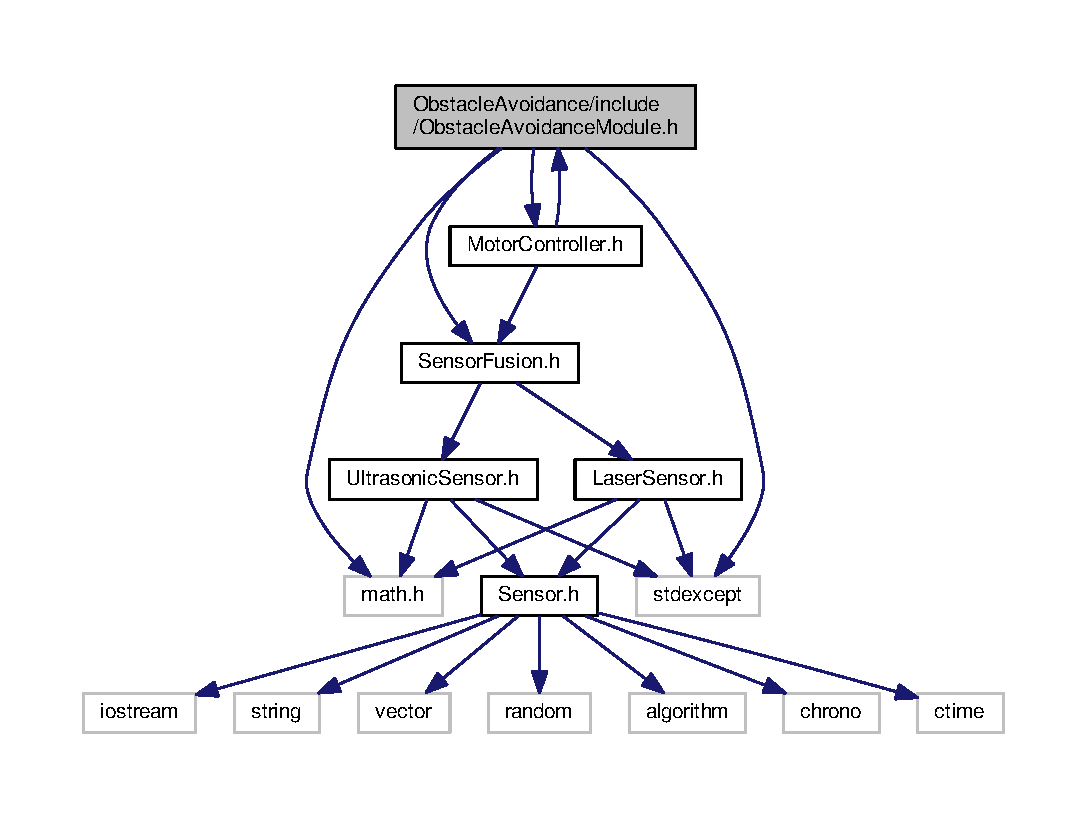
\includegraphics[width=350pt]{ObstacleAvoidanceModule_8h__incl}
\end{center}
\end{figure}
This graph shows which files directly or indirectly include this file\-:
\nopagebreak
\begin{figure}[H]
\begin{center}
\leavevmode
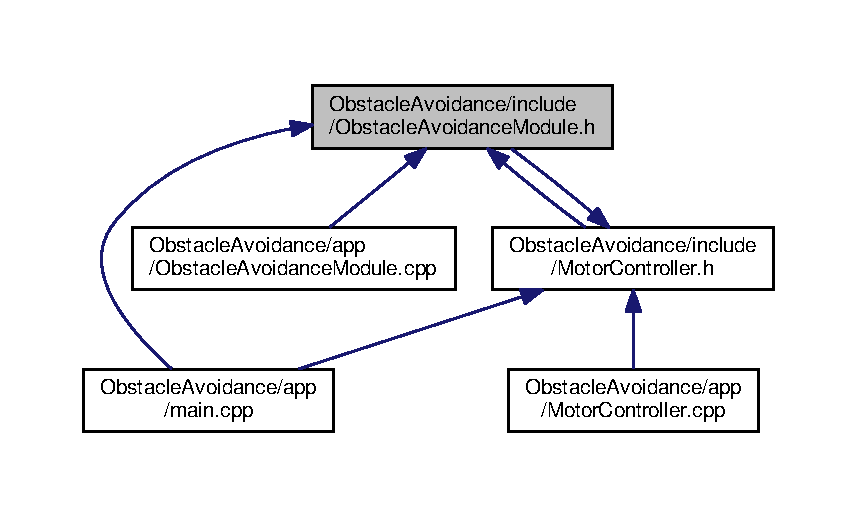
\includegraphics[width=350pt]{ObstacleAvoidanceModule_8h__dep__incl}
\end{center}
\end{figure}
\subsection*{Classes}
\begin{DoxyCompactItemize}
\item 
class \hyperlink{classObstacleAvoidance}{Obstacle\-Avoidance}
\end{DoxyCompactItemize}


\subsection{Detailed Description}
Module that detects and avoids obstacles in the path of omnidirectional robotic vehicle. Copyright 2017 Christian Ramos

\begin{DoxyVersion}{Version}
1.\-0 
\end{DoxyVersion}
\begin{DoxyDate}{Date}
Mar 7, 2017 
\end{DoxyDate}
\begin{DoxyAuthor}{Author}
Christian Ramos 
\end{DoxyAuthor}

\hypertarget{Sensor_8h}{\section{Obstacle\-Avoidance/include/\-Sensor.h File Reference}
\label{Sensor_8h}\index{Obstacle\-Avoidance/include/\-Sensor.\-h@{Obstacle\-Avoidance/include/\-Sensor.\-h}}
}


Pure virtual sensor class from which laser and ultrasonic modules are derived.  


{\ttfamily \#include $<$iostream$>$}\\*
{\ttfamily \#include $<$string$>$}\\*
{\ttfamily \#include $<$vector$>$}\\*
{\ttfamily \#include $<$random$>$}\\*
{\ttfamily \#include $<$algorithm$>$}\\*
{\ttfamily \#include $<$chrono$>$}\\*
{\ttfamily \#include $<$ctime$>$}\\*
Include dependency graph for Sensor.\-h\-:
\nopagebreak
\begin{figure}[H]
\begin{center}
\leavevmode
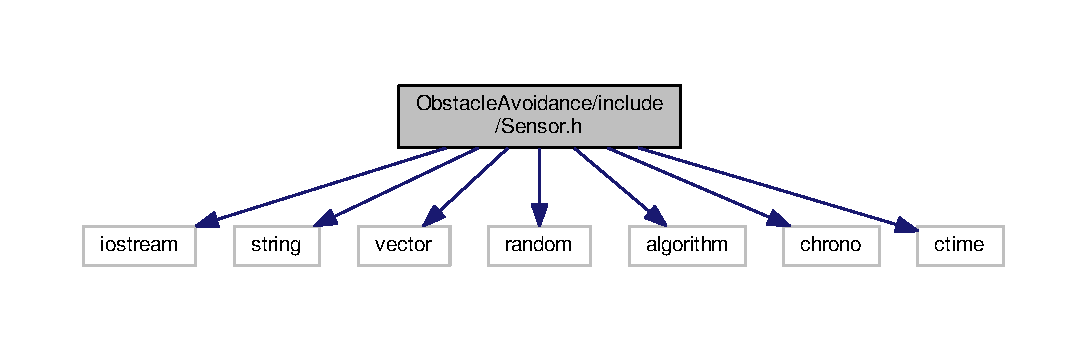
\includegraphics[width=350pt]{Sensor_8h__incl}
\end{center}
\end{figure}
This graph shows which files directly or indirectly include this file\-:
\nopagebreak
\begin{figure}[H]
\begin{center}
\leavevmode
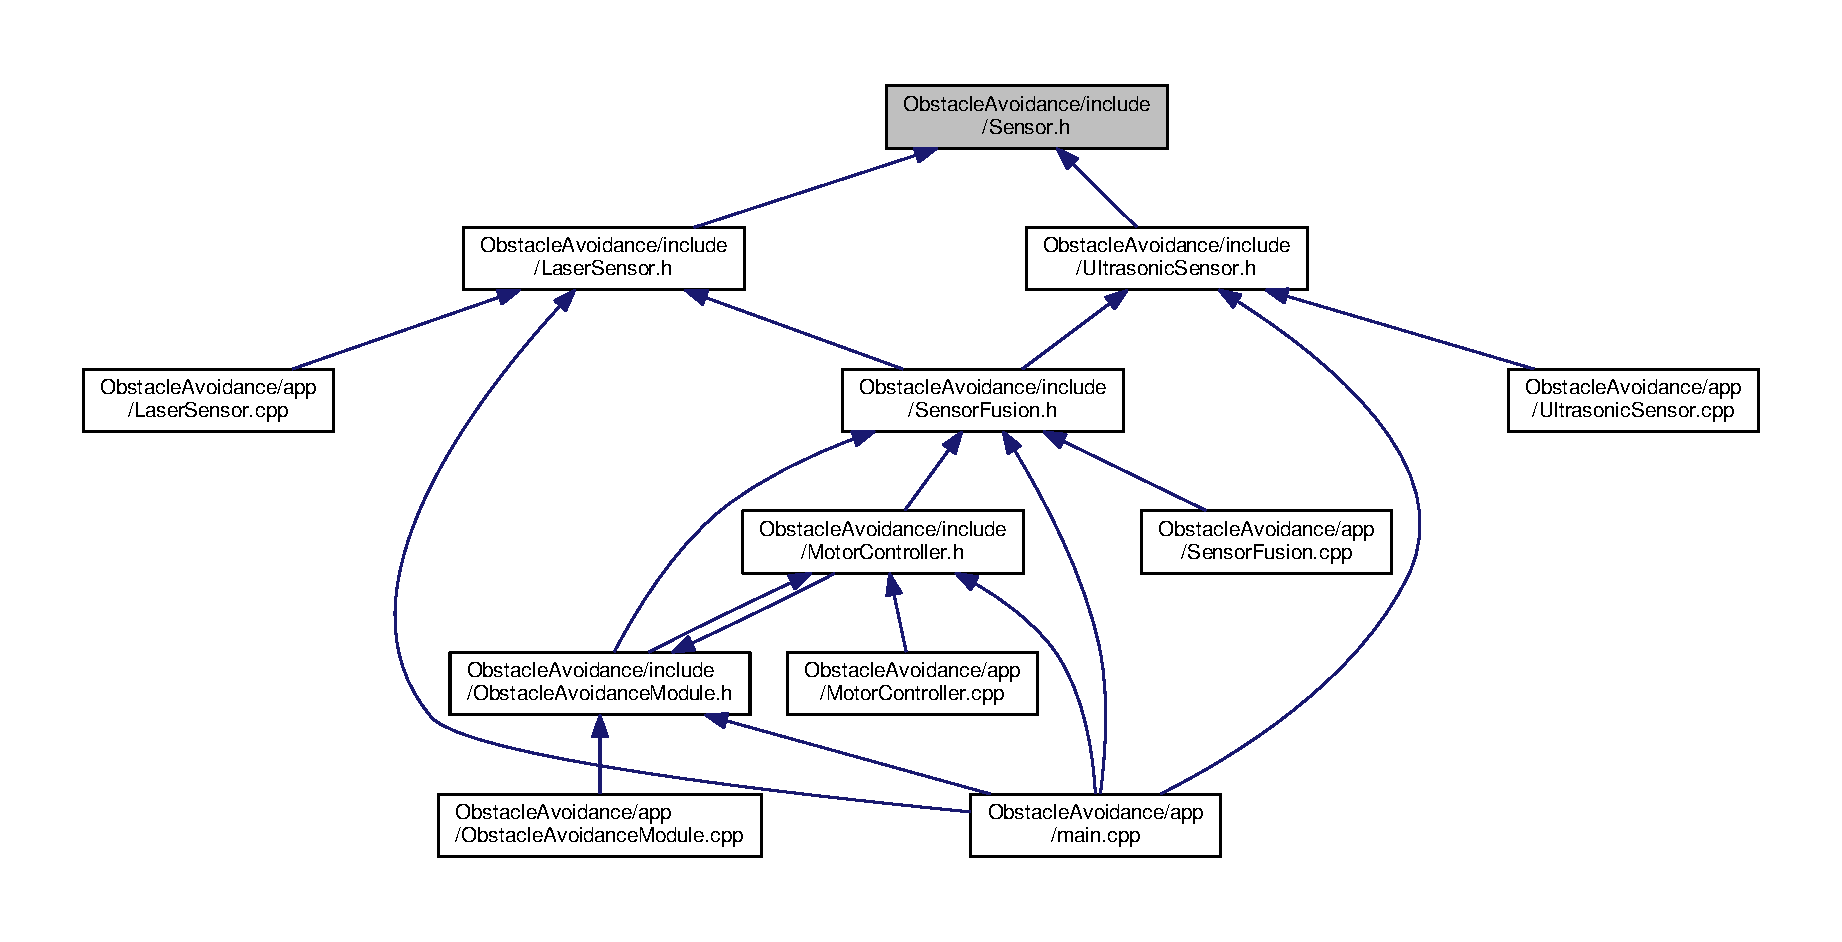
\includegraphics[width=350pt]{Sensor_8h__dep__incl}
\end{center}
\end{figure}
\subsection*{Classes}
\begin{DoxyCompactItemize}
\item 
class \hyperlink{classSensor}{Sensor}
\end{DoxyCompactItemize}


\subsection{Detailed Description}
Pure virtual sensor class from which laser and ultrasonic modules are derived. Copyright 2017 Christian Ramos

\begin{DoxyVersion}{Version}
1.\-0 
\end{DoxyVersion}
\begin{DoxyDate}{Date}
Mar 6, 2017 
\end{DoxyDate}
\begin{DoxyAuthor}{Author}
Christian Ramos 
\end{DoxyAuthor}

\hypertarget{SensorFusion_8h}{\section{Obstacle\-Avoidance/include/\-Sensor\-Fusion.h File Reference}
\label{SensorFusion_8h}\index{Obstacle\-Avoidance/include/\-Sensor\-Fusion.\-h@{Obstacle\-Avoidance/include/\-Sensor\-Fusion.\-h}}
}


Module that combines the data received from ultrasonic and laser sensors into a single averaged data set.  


{\ttfamily \#include \char`\"{}Ultrasonic\-Sensor.\-h\char`\"{}}\\*
{\ttfamily \#include \char`\"{}Laser\-Sensor.\-h\char`\"{}}\\*
Include dependency graph for Sensor\-Fusion.\-h\-:
\nopagebreak
\begin{figure}[H]
\begin{center}
\leavevmode
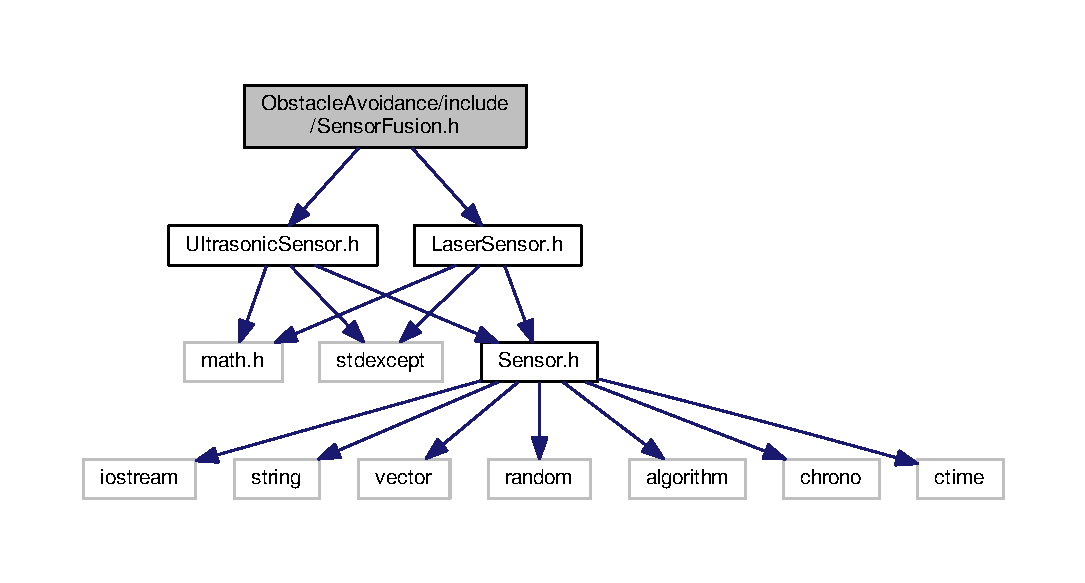
\includegraphics[width=350pt]{SensorFusion_8h__incl}
\end{center}
\end{figure}
This graph shows which files directly or indirectly include this file\-:
\nopagebreak
\begin{figure}[H]
\begin{center}
\leavevmode
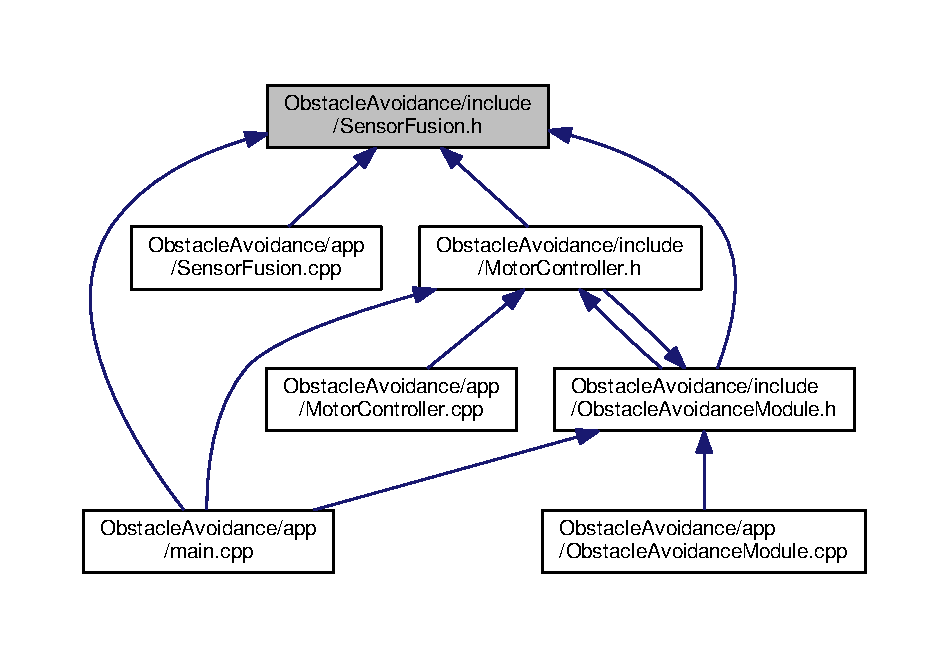
\includegraphics[width=350pt]{SensorFusion_8h__dep__incl}
\end{center}
\end{figure}
\subsection*{Classes}
\begin{DoxyCompactItemize}
\item 
class \hyperlink{classSensorFusion}{Sensor\-Fusion}
\end{DoxyCompactItemize}


\subsection{Detailed Description}
Module that combines the data received from ultrasonic and laser sensors into a single averaged data set. Copyright 2017 Christian Ramos

\begin{DoxyVersion}{Version}
1.\-0 
\end{DoxyVersion}
\begin{DoxyDate}{Date}
Mar 7, 2017 
\end{DoxyDate}
\begin{DoxyAuthor}{Author}
Christian Ramos 
\end{DoxyAuthor}

\hypertarget{UltrasonicSensor_8h}{\section{Obstacle\-Avoidance/include/\-Ultrasonic\-Sensor.h File Reference}
\label{UltrasonicSensor_8h}\index{Obstacle\-Avoidance/include/\-Ultrasonic\-Sensor.\-h@{Obstacle\-Avoidance/include/\-Ultrasonic\-Sensor.\-h}}
}


Simulates an ultrasonic sensor driver and generates laser sensor data.  


{\ttfamily \#include $<$math.\-h$>$}\\*
{\ttfamily \#include $<$stdexcept$>$}\\*
{\ttfamily \#include \char`\"{}Sensor.\-h\char`\"{}}\\*
Include dependency graph for Ultrasonic\-Sensor.\-h\-:
\nopagebreak
\begin{figure}[H]
\begin{center}
\leavevmode
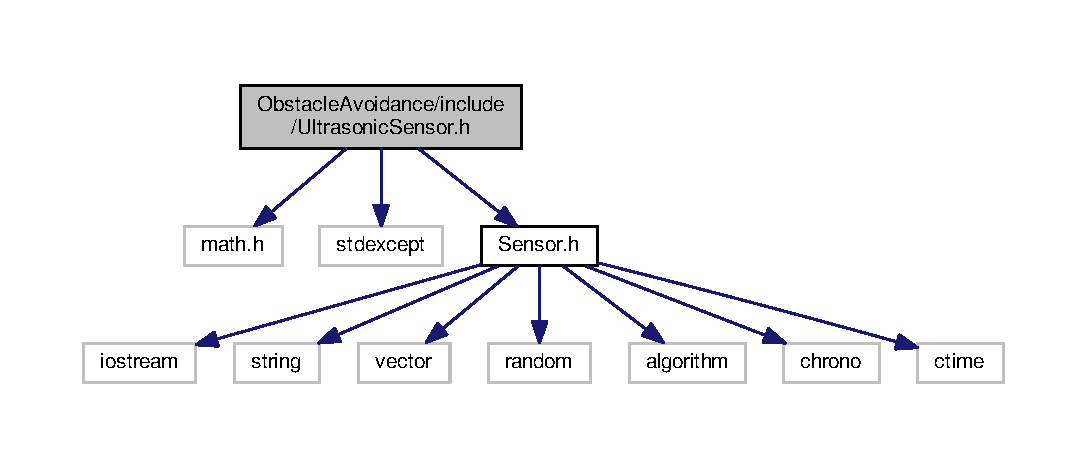
\includegraphics[width=350pt]{UltrasonicSensor_8h__incl}
\end{center}
\end{figure}
This graph shows which files directly or indirectly include this file\-:
\nopagebreak
\begin{figure}[H]
\begin{center}
\leavevmode
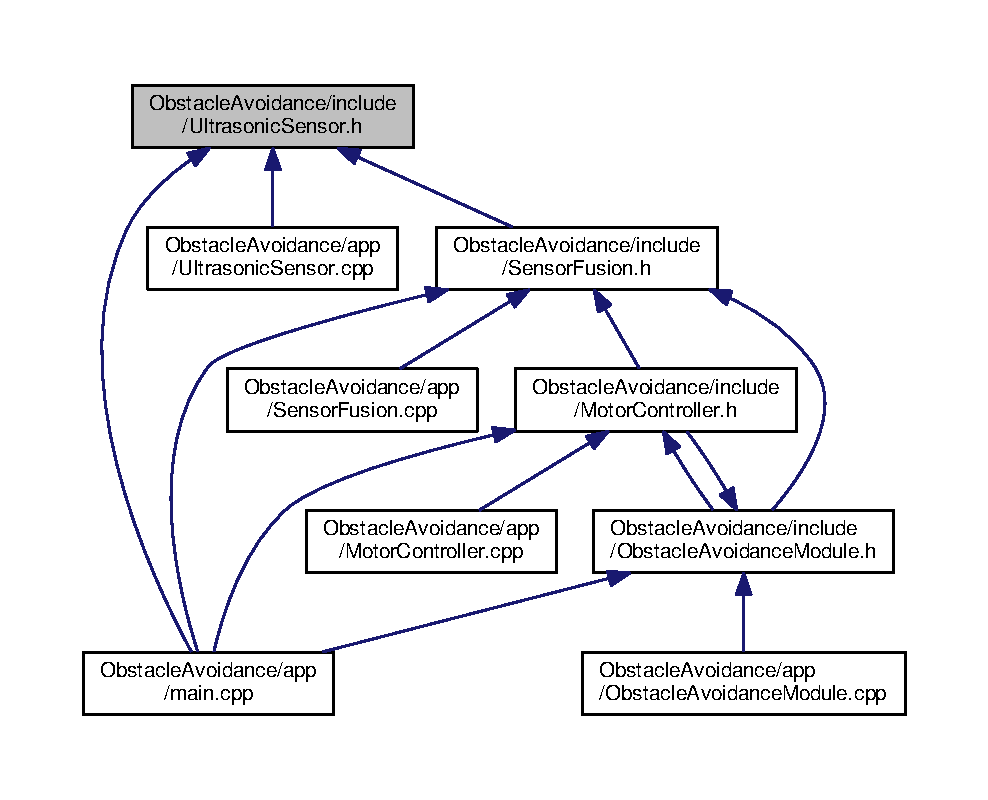
\includegraphics[width=350pt]{UltrasonicSensor_8h__dep__incl}
\end{center}
\end{figure}
\subsection*{Classes}
\begin{DoxyCompactItemize}
\item 
class \hyperlink{classUltrasonicSensor}{Ultrasonic\-Sensor}
\end{DoxyCompactItemize}


\subsection{Detailed Description}
Simulates an ultrasonic sensor driver and generates laser sensor data. Copyright 2017 Christian Ramos

\begin{DoxyVersion}{Version}
1.\-0 
\end{DoxyVersion}
\begin{DoxyDate}{Date}
Mar 6, 2017 
\end{DoxyDate}
\begin{DoxyAuthor}{Author}
Christian Ramos 
\end{DoxyAuthor}

%--- End generated contents ---

% Index
\newpage
\phantomsection
\addcontentsline{toc}{chapter}{Index}
\printindex

\end{document}
